% !TEX encoding = UTF-8 Unicode
\documentclass[12pt]{report}
\usepackage[utf8]{inputenc}
\usepackage{graphicx}
\graphicspath{ {images/} }
% header
\usepackage{fancyhdr}
\pagestyle{fancy}
% color
\usepackage[dvipsnames]{xcolor}
% bibliography
\usepackage{biblatex}
\addbibresource{references.bib}
% plot
\usepackage{pgfplots}
% code
\def\code#1{\texttt{#1}}
% cource code
\usepackage{listings}
% draft
%\usepackage{draftwatermark}
%\SetWatermarkText{DRAFT}
%\SetWatermarkScale{1}
% link
\usepackage{hyperref}
% flowchart
\usepackage{tikz}
\usetikzlibrary{shapes,arrows}
% from classicthesis
\RequirePackage{booktabs} % for better rules in tables
\RequirePackage{textcase} % for \MakeTextUppercase
\RequirePackage{soul}
% figure position
%\usepackage{float}
% glossary
\usepackage{glossaries}
% 3D plot
\usepgfplotslibrary{patchplots}
\usepackage[pdftex]{ocg}
\usepackage{pgfplots}
\pgfplotsset{compat=newest}
% subfigure
\usepackage{subcaption}
% caption style
\usepackage[font={it}]{caption}
% degree
\usepackage{gensymb}
\usepackage[T1]{fontenc}
\usepackage{textcomp}
% tabular
\usepackage{tabularx}
\usepackage{longtable}
% pdf include
\usepackage{pdfpages}
% figure
\usepackage{float}
% csv as table
\usepackage{csvsimple}
\makeglossaries

\newglossaryentry{eCore}{
	name={eCore},%
	description={An Epiphany core}%
}

\begin{document}

\lstdefinestyle{customc}{
  belowcaptionskip=1\baselineskip,
  breaklines=true,
  frame=L,
  xleftmargin=\parindent,
  language=C,
  showstringspaces=false,
  basicstyle=\footnotesize\ttfamily,
  keywordstyle=\bfseries\color{green!40!black},
  commentstyle=\itshape\color{purple!40!black},
  identifierstyle=\color{blue},
  stringstyle=\color{orange},
  basicstyle=\footnotesize,
}

\lstdefinestyle{customasm}{
  belowcaptionskip=1\baselineskip,
  frame=L,
  xleftmargin=\parindent,
  language=[x86masm]Assembler,
  basicstyle=\footnotesize\ttfamily,
  commentstyle=\itshape\color{purple!40!black},
}

\lstdefinestyle{custombash}{
  belowcaptionskip=1\baselineskip,
  frame=L,
  xleftmargin=\parindent,
  language=bash,
  basicstyle=\footnotesize\ttfamily,
}

\def\myTitle{Java GPU: technologies comparison}
\def\myName{Noémien Kocher}
\def\myUni{University of Applied Sciences of Western Switzerland}
\def\myDepartment{Department of computer science}
\def\mySupervisors{Kuonen Pierre, Jean Hennebert, Gon\c calves Louren\c co Marco Jos\'e, Beat Wolf}

\lstset{escapechar=@,style=customc}

\begin{titlepage}
    \begin{center}
        \large

        \hfill

        \vfill

        \begingroup
            \MakeUppercase{\myTitle} \\ \bigskip
        \endgroup

        \textsc{\myName}

        \vfill

        %\includegraphics[width=6cm]{gfx/TFZsuperellipse_bw} \\ \medskip

        %\mySubtitle \\ \medskip
        {\footnotesize A semester project} \\ \bigskip
        %\myDegree \\
        \myDepartment \\
        %\myFaculty \\
        %\vspace{1em}
        \myUni \\ %\bigskip
        {\footnotesize Fribourg, Switzerland}

        \vfill

        %\hfill
        {\footnotesize \textcopyright\ May 2016 \myName} \\ \bigskip
        {\footnotesize Supervisors: \mySupervisors}
    \end{center}
\end{titlepage}

\begin{abstract}

The last years have seen the rise of using GPU's not only for graphics computing, but also for a more global use in parallel computing. This completely new field comes with dedicated GPU's (GPGPU, Global Purpose GPU) that are not specialized anymore, but can be used to compute operations normally conducted on a CPU. Along with hardwares comes new programming technologies that enable programmers to use the GPU in their programs. This field is mainly divided between CUDA, which comes from NVIDIA, and OpenCL, which is an open standard. In this paper, we will be looking at technologies that enable programmers to perform GPU operations from Java code so as to evaluate them. The first chapter (\textit{Introduction}) will select the candidates and set the test battery. The second one (\textit{Analysis}) will evaluate the candidates according to our test battery. The third chapter (\textit{Results}) will compare the results obtained between the candidates and the last chapter (\textit{Conclusion}) will finally explain which solution is better and in which cases.

\smallskip
\noindent \textbf{Keywords.} Java, GPU, CUDA, OpenCL, Aparapi, JCuda, Benchmark

\end{abstract}

\printglossaries

\tableofcontents
\listoffigures

\chapter{Introduction}

This chapter will be focusing on defining the needs, selecting the candidates and setting up a test battery that will be used to compare the solutions.

Based on defined criteria, the test battery should be able to provide a fair comparison of the chosen solutions, giving a similar systematic test approach for each one.

The candidate selection, again based on defined criteria, should be able to rank every potential candidate based on an individual mark.

\section{Goals} \label{goals}

This project aims to compare different solutions that make GPU programming available in Java. Our measures will be based on the execution speed and ease of use.

We basically need either Java frameworks that give GPU computing access via some API's or solutions that directly convert Java bytecode so it is runnable on a GPU.

\section{Pre-analysis}

This chapter will be focused on selecting the candidates we want to use for our comparisons. Based on some criteria, we will run through each candidate (see appendix \ref{candidates}) we found and look if they are interesting enough to be chosen. Our criteria  will be :

\begin{itemize}
  \item Time since the last update
  \item Adoption level, community activity and documentation
  \item Adequacy for our needs
\end{itemize}


\subsection{Time since last update}

If available, the time since the last update will be the last commit. If there is no public SVN, repository or possibilities to find the last code commit, we will be looking at the date of the last product release. We will take the most recent date found.

\subsection{Adoption level, community activity and documentation}

For those criteria, mostly subjective, we will be looking at :

\begin{itemize}
  \item Quantity of pertinent search results in Google
  \item Commit activity (if available)
  \item Forum activity (if exists)
  \item Quantity of comments, articles and blogs found
\end{itemize}

\subsection{Adequacy}

For this criteria, we will be looking at the functionalities provided and see if it meets the needs of our project. Basically, it should be able to provide GPU computing capabilities via Java programming.

\newpage

\subsection{Pre-analysis table} \label{pre analysis}

\begin{longtable}{ | p{.15\textwidth} | p{.55\textwidth} | p{.30\textwidth} | }
  
  \hline
  
  \textbf{Time from update} & \textbf{Adoption level, community activity \& documentation} & \textbf{Adequacy} \\
  
  \hline \hline
  
  \multicolumn{3}{|l|}{\textbf{aparapi}} \\

  \hline

  3 months &
  Aparapi, developed by AMD, appears often in articles and researches. Seems to be in a very high adoption level and has a good documentation. &
  Allow GPU programming via bytecode translation for OpenCL. \\
  
  \hline \hline

  \multicolumn{3}{|l|}{\textbf{rootbeer}} \\

  \hline

  9 months &
  According to the readme on Github, it is still in a pre-production beta. It doesn't claim to offer
  a simple GPU programming tool giving an easily high speed up. Was under active development last year but
  seems to be left with no recent updates. It is having its longest time of inactivities since its beginning.
  Documentation not very elaborated. &
  Allow GPU programming by converting bytecode to CUDA programs. \\
  
  \hline \hline
  
  \multicolumn{3}{|l|}{\textbf{java-gpu}} \\

  \hline

  6 years &
  Doesn't seem to be maintained anymore. Has no documentation and no recent version. &
  Allow GPU programming by translating bytecode into CUDA code. \\
  
  \hline \hline
  
  \multicolumn{3}{|l|}{\textbf{ScalaCL}} \\

  \hline

  A year &
  Development stopped a year ago. Not actively maintained, seems to be dying. &
  Offers GPU programming via Scala and not directly with Java. \\
  
  \hline \hline
  
  \multicolumn{3}{|l|}{\textbf{JavaCL}} \\

  \hline

  6 months &
  Has a decent documentation but no recent activities this past years. The activities graph on github seems to show 
  that the project is dying. &
  An OpenCL wrapper for Java. \\
  
  \hline \newpage \hline
  
  \multicolumn{3}{|l|}{\textbf{jocl}} \\

  \hline

  A year &
  It has its own website and forum, which is not actively used (only 1 post this year so far). Doesn't seem
  to have a solid documentation. &
  Java binding 1:1 mapping to OpenCL \\
  
  \hline \hline
  
  \multicolumn{3}{|l|}{\textbf{lwjgl}} \\

  \hline

  today &
  It is a popular framework with a solid documentation and an active forum. &
  This is a game framework that is not primarily suited for GPU programming. \\
  
  \hline \hline
  
  \multicolumn{3}{|l|}{\textbf{jcuda}} \\

  \hline

  Last month &
  Has it's own website and forum, which is not very active. Has some tutorials and an api documentation that seems well. &
  Translate special Java code to CUDA-C. \\
  
  \hline \hline
  
  \multicolumn{3}{|l|}{\textbf{jacc}} \\

  \hline

  This year &
  Is not available and still under development. &
  Java framework that performs on low-level at runtime to use the GPU. \\
  
  \hline \hline
  
  \multicolumn{3}{|l|}{\textbf{CUDA4J}} \\

  \hline

  Last year &
  Is updated to Java 8 and developed by IBM, which certainly means a long time support. &
  Java programming API that uses lambdas and streams. \\
  
  \hline \hline
  
  \multicolumn{3}{|l|}{\textbf{PJ2}} \\

  \hline

  Last month &
  It is an API developed at the Rochester Institute. It is still under maintenance but doesn't have
  a community and is not really well known. &
  Middleware API for Java programming on multicore platforms. \\
  
  \hline

\end{longtable}

\subsection{Grades} \label{grades}

To rank our options, we will give, based on each criteria, a grade going from 0 to 10, 10 being the best and 0 the worst.

Time from update, adoption level and adequacy grade will go according to the following tables:

\begin{center}
\captionof{table}{Grade: Time from update}
\begin{tabular}{|c|c|c|c|c|}
	\hline
	< 3 months & < 6 months & < 1 years & < 2 years & > 2 years \\
	\hline
	10 & 8 & 5 & 3 & 0 \\
	\hline
\end{tabular}
\end{center}

\begin{center}
\captionof{table}{Grade: Adoption level, community activity and documentation}
\begin{tabular}{|p{.25\textwidth}|p{.25\textwidth}|p{.25\textwidth}|p{.25\textwidth}|}
	\hline
	Is well referenced, found many articles and is well documented & 
	Appears quite often in a google search, found some articles and has a fairly good documentation &
	Found some results in a google search and has a documentation &
	Didn't found much results in a google search, has a poor documentation \\
	\hline
	10 & 8 & 5 & 3 \\
	\hline
\end{tabular}
\end{center}

\begin{center}
\captionof{table}{Grade: Adequacy}
\begin{tabular}{|p{.25\textwidth}|p{.25\textwidth}|p{.25\textwidth}|p{.25\textwidth}|}
	\hline
	Fits perfectly our needs & 
	Fits partially our needs, or the solution is not aimed to particularly fits out needs &
	Doesn't fit our needs \\
	\hline
	10 & 3 & 0 \\
	\hline
\end{tabular}
\end{center}

\subsection{Grades table}

According to our pre-analysis (see section \ref{pre analysis}) and our grades (section \ref{grades}), each candidates has been evaluated and got a corresponding mark. Based on the marks, we will choose the candidates that have the highest ones.

\begin{longtable}{ | p{.20\textwidth} | p{.20\textwidth} | p{.20\textwidth} | p{.20\textwidth} | p{.10\textwidth} | }
  
  \hline
  
  & Time from update & Adoption level, community activity \& documenation & Adequacy & \textbf{Grade} \\
  
  \hline \hline
  
  \textbf{aparapi} &
  10 &
  10 &
  10 &
  \textbf{30} \\
  
  \hline \hline
  
  \textbf{jcuda} &
  10 &
  8 &
  10 &
  \textbf{28} \\
  
  \hline \hline
  
  \textbf{CUDA4J} &
  5 &
  10 &
  10 &
  \textbf{25} \\
  
  \hline \hline
 
  \textbf{PJ2} &
  10 &
  5 &
  10 &
  \textbf{25} \\
  
  \hline \hline

  \textbf{rootbeer} &
  5 &
  8 &
  10 & 
  \textbf{23} \\
  
  \hline \hline
  
  \textbf{java-gpu} &
  8 &
  5 &
  10 &
  \textbf{23} \\
  
  \hline \hline
  
  \textbf{JavaCL} &
  8 &
  5 &
  10 &
  \textbf{23} \\
  
  \hline \hline
  
  \textbf{lwjgl} &
  10 &
  10 &
  3 &
  \textbf{23} \\
  
  \hline \hline
  
  \textbf{jacc} &
  5 &
  5 &
  10 &
  \textbf{20} \\
  
  \hline \hline
  
  \textbf{jocl} &
  5 &
  5 &
  10 &
  20 \\
  
  \hline \hline
  
  \textbf{ScalaCL} &
  5 &
  5 &
  10 &
  20 \\
  
  \hline

\end{longtable}

\section{Nominees}

Based on our prior analysis, we will only be focusing on the first two technologies, which obtained the highest grades with 30/30 for Aparapi and 28/30 for JCuda. Those technologies will give us the opportunity to test an openCL and CUDA based solution.


\section{Battery of tests} \label{battery test}

Testing our solution will require us to write a first implementation using vanilla Java code, then writing two other implementations - still in Java - but adapted to use a specific solution (in our case, it will be Aparapi and JCuda). We will then be able to compare the implementations.

We will base our tests on two main aspects :

\begin{enumerate}
  \item Speed
  \item Ease of use
\end{enumerate}

\textbf{1: The first aspect - Speed -} will use some benchmarks code testing specific computation aspects like floating point operations or integer manipulations. Those tests will give us precise metrics that will be easily comparable.

\textbf{2: The second aspect - ease of use -} are more kind of subjective and will need a systematic approach so as to be the most fair. We will be looking at some defined criteria, like the number of code lines and the programmer's feedback. The next section will discuse in more details the two aspects.

\subsection{Speed} \label{subsection speed}

To add more relevance to our benchmark, we wanted to choose two benchmarks that does not perform the same type of operations. The most obvious one - a matrix computation - was our first choice. Due to its simple implementation and its ability to be distributed on different cores, we rapidly opted for this one. The matrix multiplication will be able to measure floating point manipulations performance. 

Our second choice was to make an array sorting. But, after testing some pieces of code, we went back and looked for another alternative. The idea of the array sorting, as shown in figure \ref{fig sort}, was to split the array, distribute the subsets and perform a merge sort. This solution was simple to code but performed very badly concerning memory space.

\begin{figure}[h!]
\centering
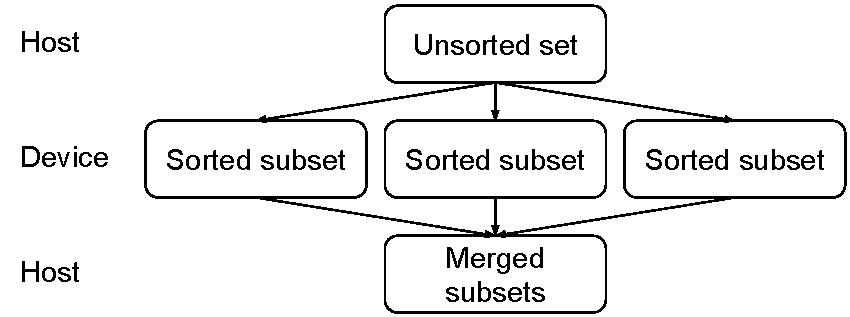
\includegraphics[width=0.7\textwidth]{sort}
\caption{Sorting principle}
\label{fig sort}
\end{figure}

We then looked for the prime factorization of an integer. Again, quite easy to code (see figure \ref{listing factor}), but this time our implementation wasn't suited to be ported on a multi-threaded architecture and was highly limited by Java integer size, even using \textit{BigInteger}.

\begin{figure}
	\begin{lstlisting}
BigInteger n = 999999;
BigInteger i = new BigInteger("2");
for(; i.compareTo(n.divide(i)) <= 0; i = i.add(BigInteger.ONE)) {
  while(n.mod(i).equals(BigInteger.ZERO)) {
    System.out.println("Divisor: " + n);
    n = n.divide(i);
  }
}
	\end{lstlisting}
\caption{Factorization of a number}
\label{listing factor}
\end{figure}

We finally opted for the computation of a Levenshtein distance between two strings. The code remains simple, is not heavily restrained by variables' size and can be adapted to a multi-threaded architecture.

To summarize, the speed measure will be based on those two simple computation operations :

\begin{enumerate}
  \item A matrix multiplication using floating variables
  \item Levenshtein distance computation of two strings
\end{enumerate}

\textbf{1: The matrix multiplication} will be as simple as possible, using the basic definition saying that each cell of the resulting matrix $C {{=}} AB$ is given by the following formula :

\begin{equation}
	c_{ij} = \sum_{k=1}^m a_{ik} b_{kj}
\end{equation}

This method leads to a complexity of $O(n^3)$ for a squared matrix of size $n$, which is fine for a benchmark purpose. To have a code as flexible as possible, we won't use any Java matrix objects, but only 2-dimensions doubles arrays. figure \ref{listing matrix} shows a sample code of the matrix multiplication.

\begin{figure}[h!]
\begin{lstlisting}
  // Computes matrix multiplication C = AB
  public static void matrixMul(double[][] A, double[][] B, 
                               double[][] C) {
    for(int i=0; i < size; i++) {
      for(int j=0; j < size; j++) {
        double sum = 0.0;
        for(int k=0; k < size; k++) {
          sum += A[i][k] * B[k][j];
        }
        C[i][j] = sum;
      }
    }
  }
\end{lstlisting}
\caption{Sample code of the matrix multiplication}
\label{listing matrix}
\end{figure}

Adapting the code on a multithreaded architecture won't be difficult since each cell, row or column can be computed independently on a separate core.

The matrix content will be randomized and adjusted according to the matrix size so as to prevent overflows. The size will be set to produce a computation time from 30 seconds to 1 minute. The random seed will be the same among all our tests so as to keep the same conditions.

Figure \ref{fig plot matrix} is a quick single measure of the complexity scale of our implementation. The result has been compared to other same measures so as to ensure that there is no edge cases or noise in our results. Raw values of this measure are available in the appendix \ref{raw values quick matrix}, and the comparison made with another measure can be found in the appendix \ref{vanilla matrix both}.

\begin{figure}[h!]
\centering
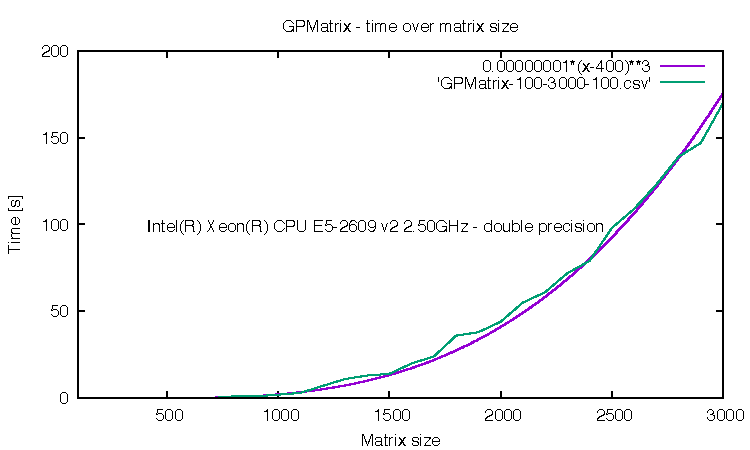
\includegraphics[width=1\textwidth]{vanillaPlotMatrix}
\caption{Complexity scale of the matrix implementation}
\label{fig plot matrix}
\end{figure}


\textbf{2: The Levenshtein distance} will be based on the definition found on wikipedia\cite{levenshteinwiki} stating that:

$\qquad\operatorname{lev}_{a,b}(i,j) = \begin{cases}
  \max(i,j) & \text{ if} \min(i,j)=0, \\
  \min \begin{cases}
          \operatorname{lev}_{a,b}(i-1,j) + 1 \\
          \operatorname{lev}_{a,b}(i,j-1) + 1 \\
          \operatorname{lev}_{a,b}(i-1,j-1) + 1_{(a_i \neq b_j)}
       \end{cases} & \text{ otherwise.}
\end{cases}$

 We will use an already existing implementation\cite{levenshtein} that will be adapted for a multi-threaded use.
The strings will be generated randomly and the size will be adjusted to give a computation time from 30 seconds to 1 minute. The strings will be stored in files. It has the advantages of being reusable and not limited by the maximum Java string size or input parameter size. The listing \ref{listing leven} is a sample code computing the Levenstein distance. This is the one that will be adapted to be used on the GPU.

\begin{figure}[h!]
\begin{lstlisting}
  public static int distance(String a, String b) {
    int [] costs = new int [b.length() + 1];
    for (int j = 0; j < costs.length; j++)
      costs[j] = j;
    for (int i = 1; i <= a.length(); i++) {
      costs[0] = i;
      computeRow(costs, i, a, b);
    }
    return costs[b.length()];
  }

  // Compute a single row in the distance process
  public static void computeRow(int[] costs, int i, String a, String b) {
    int nw = i - 1;
    for (int j = 1; j <= b.length(); j++) {
      int cj = Math.min(1 + Math.min(costs[j], costs[j - 1]), a.charAt(i - 1) == b.charAt(j - 1) ? nw : nw + 1);
      nw = costs[j];
      costs[j] = cj;
    }
  }
\end{lstlisting}
\caption{Sample code of the Levenstein distance computation}
\label{listing leven}
\end{figure}


Figure \ref{fig plot leven} is a measure of the complexity scale of the implementation. We took an average based on 5 executions. In this case, we observe a complexity of $O(n^2)$, which grows much less than the matrix multiplication. Raw values of this measure can be found in the appendix \ref{raw values quick leven}.

\begin{figure}[h!]
\centering
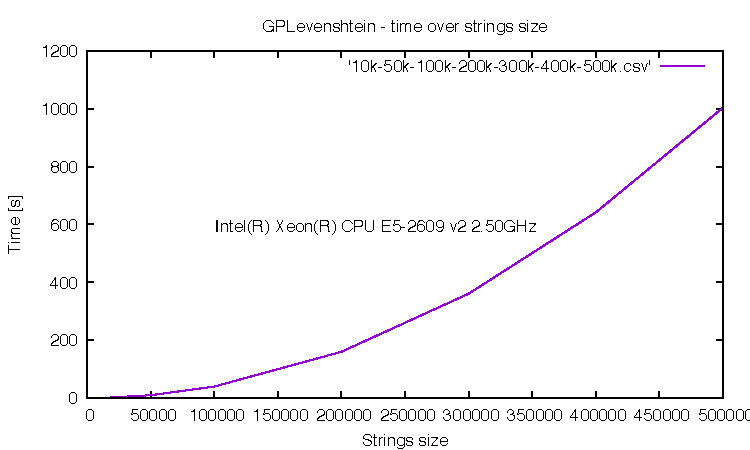
\includegraphics[width=1\textwidth]{vanillaPlotLeven2}
\caption{Complexity scale of the Levenshtein implementation, average on 5 executions}
\label{fig plot leven}
\end{figure}

\subsection{Ease of use}

To measure the ease of use, we will be looking at :

\begin{enumerate}
  \item The number of line codes (LOC)
  \item A personal feedback after the solution's installation
  \item External reviews of the code by some developers
  \item A personal feedback after the execution of the test battery
\end{enumerate}

\textbf{1: The line of codes} will be taken from the routines performing the speed tests mentioned in the previous subsection (\ref{subsection speed}). Each routine will be evaluated separately and compared to the other implementations. We won't take blank lines and comments into account.

\textbf{2: The personal feedback} will be written right after the setting up of the solution. This feedback will evaluate if the solution is hard to set up or easily usable, like an out-of-the box solution. The environment will already have CUDA and OpenCL set up, so that part will not be evaluated.

\textbf{3: Having an external review} from some developers will help having a fresh point of view. While developing and judging his own code can alter an opinion, someone external will have a neat more objective point of view concerning the complexity of a code. Those persons will be asked to understand the code and give a grade from 1 (very hard) to 5 (very easy) about how it is hard or not to understand how the code uses the GPU.

\textbf{4: The personal conclusion} will be a conclusion after the end of the test battery. It will give an overall feedback about the setting up and development with a particular solution.

\subsection{Test process}

Figure \ref{fig tprocess} shows the sequential process that will be applied for our test battery.

\begin{figure}[h!]
\centering
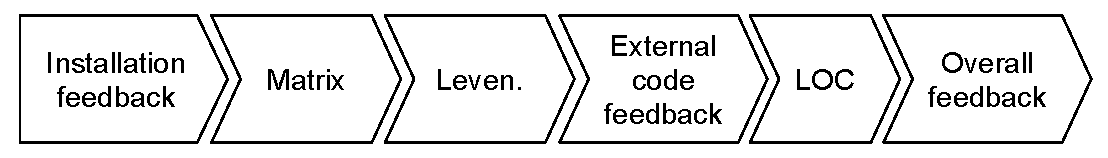
\includegraphics[width=1\textwidth]{testprocess}
\caption{Testing process}
\label{fig tprocess}
\end{figure}

\chapter{Analysis}
This chapter will evaluate Aparapi and JCuda - the two candidates who have got the highest marks - based on the test battery discussed in the previous chapter. At the end of this chapter, we will be able to compare the two solutions. This chapter will only be focusing on analyzing the solutions and the comparison between Aparapi and JCuda will come in the next chapter.

\section{Aparapi}

This section will evaluate Aparapi according to the test battery discussed in section \ref{battery test}.

Aparapi stands for A PAR\{allel\} API. It is a tool developed by AMD that gives the ability to write Java code for the GPU. Aparapi works with any configuration supporting a compatible OpenCL 1.1 runtime \cite{aparapiquestions}.

To be able to send GPU jobs, Aparapi dynamically translates Java bytecode at runtime to OpenCL instructions \cite{aparapiblog}. This makes the process of using Aparapi very transparent from the developer's point of view.

\subsection{Installation}

Using Aparapi only requires to include a library jar at the compilation stage and at the execution time. Once done, one can use the Aparapi's API to write specific GPU code.

The jar library comes with several examples that shows how to compile and write code. While we couldn't easily found a getting started guide, but we rapidly understood the process reading some examples.

Aparapi doesn't need any software installation except having a working OpenCL runtime. It only requires to include a jar in the compilation and execution stages and setting up the correct LD\_LIBRARY\_PATH containing the shared object (.so) library.

The following code shows a typical compilation and run process :

\begin{lstlisting}
$ javac -cp aparapi.jar:. GPLevenshtein.java
$ java -cp aparapi.jar:. GPLevenshtein 1000
\end{lstlisting}

The next listing shows how we included the shared object library:

\begin{lstlisting}
$ export LD_LIBRARY_PATH=$LD_LIBRARY_PATH:/path/to/foler
\end{lstlisting}

The process of using Aparapi is nearly the same as writing CPU threads \cite{aparapiarticle}. Basically, the kernel method will be in a class that inherits from Aparapi's Kernel class. The kernel method is called a given number of times when the class is instantiated. The following example uses Aparapi to perform the addition of two vectors:

\begin{lstlisting}
// The following class contains the kernel method that
// sums two vectors.
// The following code would runs the kernel :
// new AparapiLevenshtein(a,b,result).execute(a.length);
class AparapiExample extends Kernel {
  int[] a;
  int[] b;
  int[] result;
  
  public AparapiLevenshtein(int[] a, int[] b, int[] result) {
    this.a = a;
    this.b = b;
    this.result = result;
  }

  // Kernel method
  public void run() {
    int i = getGlobalId(); // The thread id
    result[i] = a[i] + b[i];
  }
}

\end{lstlisting}

\subsection{Matrix multiplication}

The code computing the matrix multiplication with Aparapi can be found in the appendix \ref{aparapi code}.

As seen in figure \ref{fig plot matrix aparapi}, aparapi gives a speedup up to 6 compared to a vanilla execution. It is interesting to note that the speedup is not constant over the matrix size (uncertainty may be the reason, see appendix \ref{uncertain}), but seems to stagnate around 5. The raw values of the speedup are available in the appendix \ref{raw values speedup aparapi matrix} and the uncertainty is discussed in appendix \ref{uncertain}.

\begin{figure}[H]
\centering
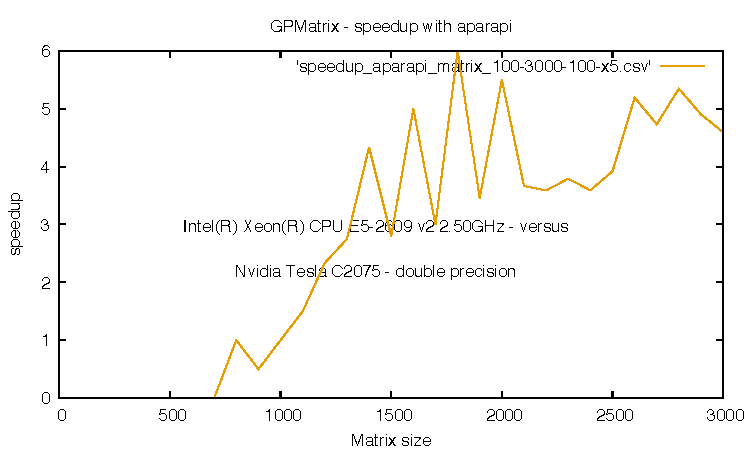
\includegraphics[width=1\textwidth]{speedup_aparapi_matrix_5x.pdf}
\caption{Speedup gained using Aparapi on matrix multiplication}
\label{fig plot matrix aparapi}
\end{figure}

Figure \ref{fig: plot aparapi matrix times} gives us sequential time running the matrix computation using vanilla Java and Aparapi. For each measure we took the average of 5 executions. We observe that using Aparapi on a GPU doesn't give a smooth curve. Those perturbations could be due to the operating system resource usages during the measures, but we didn't perform any other operations than executing the benchmark and repeated the measures 5 times. It is is probably due the rounding (see appendix \ref{uncertain}). The raw values of the sequential times using Aparapi on the matrix multiplication are available in the appendix \ref{raw values aparapi matrix}.

\begin{figure}[H]
\centering
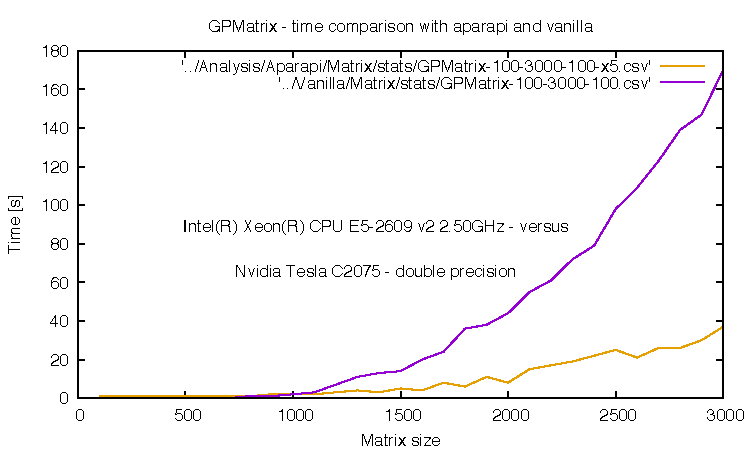
\includegraphics[width=1\textwidth]{time_aparapi_matrix_5x.pdf}
\caption{Times over matrix size using vanilla Java and Aparapi}
\label{fig: plot aparapi matrix times}
\end{figure}

Figure \ref{fig table matrix aparapi} gives some statistics about the speedup gained with our measures. Those metrics are specifics but, as will the others, it will give us the ability to compare them against another solution - like JCuda.

\begin{figure}[H]
\begin{center}
\begin{tabular}{ |l|l| } 
 \hline
 Speedup average & 2,3 \\ 
 Speedup median & 3.4 \\ 
 Speedup std. deviation & 1,8 \\ 
 \hline
\end{tabular}
\end{center}
\caption{Speedup statistics of matrix multiplication performed with Aparapi}
\label{fig table matrix aparapi}
\end{figure}

\subsection{Levenshtein distance}

The code computing the Levenshtein distance with Aparapi can be found in the appendix \ref{aparapi code}.

As seen in figure \ref{fig plot leven aparapi}, the speedup is at its best with a string size around 200'000 characters. Between this value, the speedup decreases. It is interesting to note that two different types of computation gives a significantly different speedup tendency. In this case, the algorithm is only really efficient around a specific string size range. The raw values of the speedup are available in the appendix \ref{raw values speedup aparapi Leven} and the uncertainty is discussed in appendix \ref{uncertain}.

\begin{figure}[H]
\centering
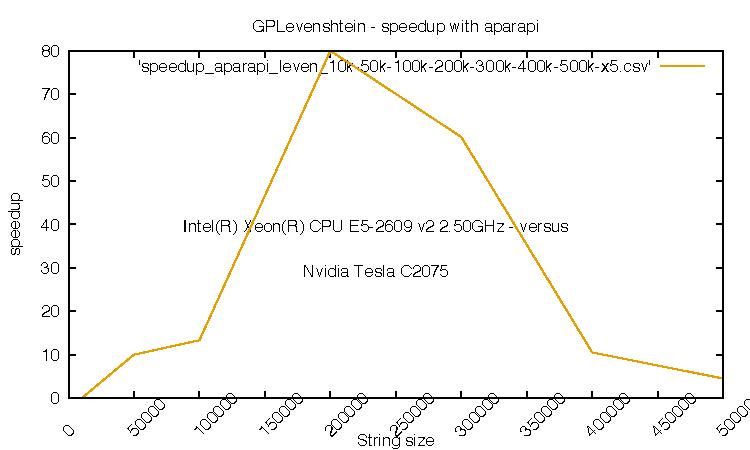
\includegraphics[width=1\textwidth]{speedup_aparapi_leven_5x.pdf}
\caption{Speedup gained using Aparapi on levenstein computation}
\label{fig plot leven aparapi}
\end{figure}

Figure \ref{fig: plot aparapi leven times} shows sequential time while running levenstein computation on a vanilla implementation and using Aparapi. We can observe that those curves have the same tendency and, around 200'000, show a small decreasing time for the Aparapi execution, thus giving the kind of 'mountain' for the speedup. Raw values of the sequential time using Aparapi for the Levenshtein distance computation is available in the appendix \ref{raw values aparapi leven}.

\begin{figure}[H]
\centering
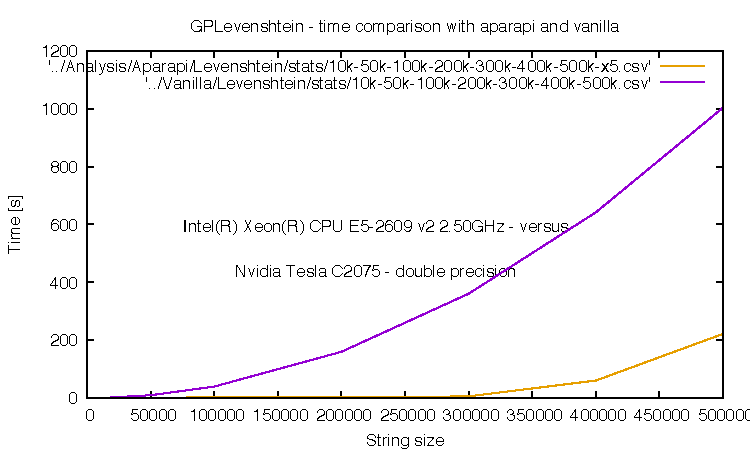
\includegraphics[width=1\textwidth]{time_aparapi_leven_5x.pdf}
\caption{Times over string sizes using java and Aparapi}
\label{fig: plot aparapi leven times}
\end{figure}

Figure \ref{fig table leven aparapi} shows some statistics of the speedup gained with our measures. As observed in figure \ref{fig plot leven aparapi}, we come with a high standard derivation, due to the kind of 'mountain' we obtained in our graph.

\begin{figure}[H]
\begin{center}
\begin{tabular}{ |l|l| } 
 \hline
 Speedup average & 25,2 \\ 
 Speedup median & 10 \\ 
 Speedup std. deviation & 29 \\ 
 \hline
\end{tabular}
\end{center}
\caption{Speedup statistics of levenstein computation performed with Aparapi}
\label{fig table leven aparapi}
\end{figure}

\subsection{External code feedback}

We asked 2 developers to evaluate the difficulty of using Aparapi to write GPU code. We gave them the Matrix multiplication and the Levenshtein distance source codes asking them to give a mark from 1 (very difficult to understand) to 5 (very easy to understand). The surveys can be found in the appendix \ref{aparapi code}.

Results are given in figure \ref{table aparapi code feedback}:

\begin{figure}[H]
\begin{center}
\begin{tabular}{ |l|l|l|l| } 
 \hline
  & \textbf{Matrix} & \textbf{Levenstein} \\
 \hline
 \textbf{Developper 1} & 5 & 5 \\ 
 \hline
 \textbf{Developper 2} & 5 & 5 \\ 
 \hline
\end{tabular}
\end{center}
\caption{Results of the Aparapi surveys. From 1 (very difficult to understand) to 5 (very easy to understand)}
\label{table aparapi code feedback}
\end{figure}

\subsection{LOC}

The number of code lines needed to use Aparapi for the matrix multiplication and Levenshtein distance computation are given in figure \ref{table aparapi loc}. Those numbers only include the methods used to compute the matrix multiplication and the Levenstein distance, removing comments and blank lines.

\begin{figure}[H]
\begin{center}
\begin{tabular}{ |l|l|l|l| } 
 \hline
 & \textbf{vanilla} & \textbf{Aparapi} & \textbf{delta} \\
 \hline
 \textbf{GPMatrix} & 13 & 21 & 8 \\ 
 \hline
 \textbf{GPLevenstein} & 18 & 24 & 6 \\ 
 \hline
\end{tabular}
\end{center}
\caption{LOC of GPMatrix and GPLevenstein using Aparapi compared to vanilla}
\label{table aparapi loc}
\end{figure}

\subsection{Overall feedback}

Installing and using Aparapi is quite straightforward. The first problem we met was to find an official documentation about installing and using Aparapi. While we couldn't find any relevant official documentation, we came up using a given example to take our first steps. Reading an example gave us enough information to start adapting our code using Aparapi.

The second problem we met was that using Java object inside the kernel function is not possible. We had to remove all Java object usages and adapt our implementation - for example by using a char array instead of a string in GPLevenstein. This restriction wasn't clearly documented by Aparapi.

The third problem we met was that getting the length of an array raised an error. After investigating, we found out that it is a know bug \cite{aparapibug}. This step took us a while to discover since the raised error wasn't explicit and didn't directly guide us to the real error's source.

In conclusion, Aparapi was quite easy to use despite the loss of an official and complete documentation. Not having the ability to use Java objects is disappointing and removes a major advantage of using Java code. But for specific uses, Aparapi is a simple and efficient solution to perform GPU computation inside Java code. 

\section{JCuda}

This section will evaluate JCuda according to the test battery discussed in section \ref{battery test}.

JCuda is a binding library that uses NVIDIA CUDA technologies. CUDA® is a parallel computing platform and programming model invented by NVIDIA. It enables dramatic increases in computing performance by harnessing the power of the graphics processing unit (GPU)\cite{cudahome}.

JCuda provides binding from Java to CUDA. The library enables programmers to write Java methods. Thoses methods will be automatically bound to the corresponding CUDA ones, which would be written in CUDAC/C++ \cite{cudagpgpu}.

With JCuda, programmers will have to write the kernel method in a separate native CUDA file (.cu) and use the JCuda library from Java to call the kernel and perform data transfers. The process is nearly similar as one would do with plain CUDA language, but using adapted Java methods.

\subsection{Installation}

The installation of JCuda requires the same process as with Aparapi. A jar library needs to be included in the compilation and execution stages and a library (shared object file on Linux) must be visible to Java at runtime (typically using LC\_LIBRARY\_PATH).

No extra software is needed, but only having a working CUDA environment setup and including the JCuda library.

The installation process is well documented as well as the first steps to write a first program using JCuda. There are also plenty of examples to help understanding how JCuda works.

A typical compilation and run case for a JCuda program would be something like :
\begin{lstlisting}
$ javac -cp ".:jcuda-0.7.5.jar" GPMatrix.java
$ java  -cp ".:jcuda-0.7.5.jar" GPMatrix 1000
\end{lstlisting}

To get an idea of how JCuda works, the following listing shows an example of a two vectors addition using JCuda :

\begin{lstlisting}
// From the Java class
  ...
  int[] A = ...; int[] B = ...;
  int[] result = ...; int size = a.length;
  
  // Create the PTX file by calling the NVCC
  String ptxFileName = preparePtxFile("kernel.ptx");
  
  // Load the CUDA kernel ptx file
  CUmodule module = new CUmodule();
  cuModuleLoad(module, ptxFileName);

  // Obtain a function pointer to the kernel function
  CUfunction function = new CUfunction();
  cuModuleGetFunction(function, module, "add");

  // Allocate the device input/output data, and 
  // copy the host input data to the device
  int ptrSize = size * Sizeof.INT;
  CUdeviceptr deviceInputA = new CUdeviceptr();
  cuMemAlloc(deviceInputA, ptrSize);
  cuMemcpyHtoD(deviceInputA, Pointer.to(A), ptrSize);

  CUdeviceptr deviceInputB = new CUdeviceptr();
  cuMemAlloc(deviceInputB, ptrSize);
  cuMemcpyHtoD(deviceInputB, Pointer.to(B), ptrSize);

  CUdeviceptr deviceOutput = new CUdeviceptr();
  cuMemAlloc(deviceOutput, ptrSize);

  // Set up the kernel parameters: A pointer to an array
  // of pointers which points to the actual values
  Pointer kernelParameters = Pointer.to(
    Pointer.to(deviceInputA),
    Pointer.to(deviceInputB),
    Pointer.to(deviceOutput),
    Pointer.to(new int[]{size})
  );

  // Kernel call parameters
  int blockSizeX = 256;
  int gridSizeX = (int)Math.ceil((double)size / blockSizeX);

  // --------------------------------
  long startTime = System.currentTimeMillis();
  // --- Start of benchmark zone --->
  cuLaunchKernel(function,
    gridSizeX, 1, 1,       // Grid dimension
    blockSizeX, 1, 1,     // Block dimension
    0, null,              // Shared memory size and stream
    kernelParameters, null // Kernel and extra parameters
  );
  cuCtxSynchronize();
  
  // Get the result
  cuMemcpyDtoH(Pointer.to(result), deviceOutput, ptrSize);
...

// Kernel.cu
extern "C"
__global__ void add(int* A, int* B, int* result, int size) {
  int i = blockIdx.x * blockDim.x + threadIdx.x;

  if(i < size) {
    result[i] = A[i] + A[i];
  }
}

\end{lstlisting}

\subsection{Matrix multiplication}

Like we did with Aparapi, we took the matrix multiplication vanilla code and ported the same portion of code as with Aparapi to the GPU. We then made the same measures as with Aparapi and computed the speedup gained between JCuda and vanilla Java code. The adapted code can be found in the appendix \ref{jcuda code}.

Figure \ref{fig plot matrix jcuda} shows the speedup gained using JCuda in the matrix multiplication code. We can see that we obtained a speedup rising up to 12. The shape of the curve is not constantly rising, but is giving a maximum around a matrix size between 2000 and 2500.

So as to prevent edge cases and removing noise, we each time took 5 measures and used the average values between the 5 results. Raw values for the speedup using JCuda on the matrix multiplication are available in the appendix \ref{raw values speedup jcuda matrix} and the uncertainty is discussed in appendix \ref{uncertain}.

\begin{figure}[H]
\centering
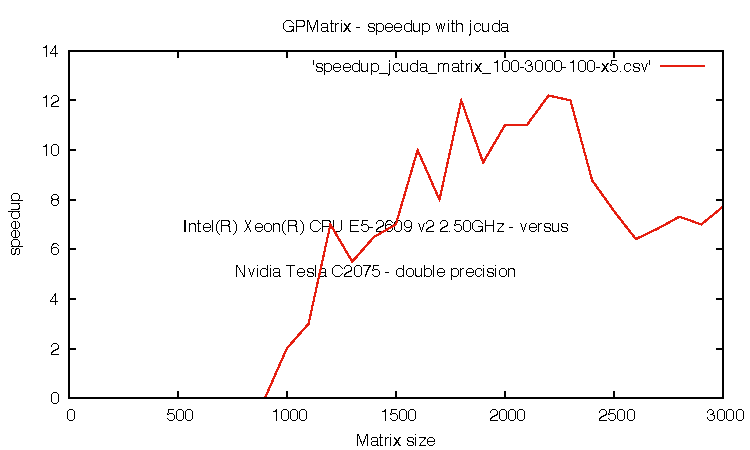
\includegraphics[width=1\textwidth]{speedup_jcuda_matrix_5x.pdf}
\caption{Speedup gained using JCuda on matrix multiplication}
\label{fig plot matrix jcuda}
\end{figure}

Figure \ref{fig: plot jcuda matrix times} gives us sequential times of the vanilla execution and the JCuda one on the matrix multiplication. The sequential times with JCuda seem to expand on a logarithm form while the sequential times on the vanilla code expand more in an exponential manner. Raw values of the sequential times using JCuda on the matrix multiplication can be found in the appendix \ref{raw values jcuda matrix}.

\begin{figure}[H]
\centering
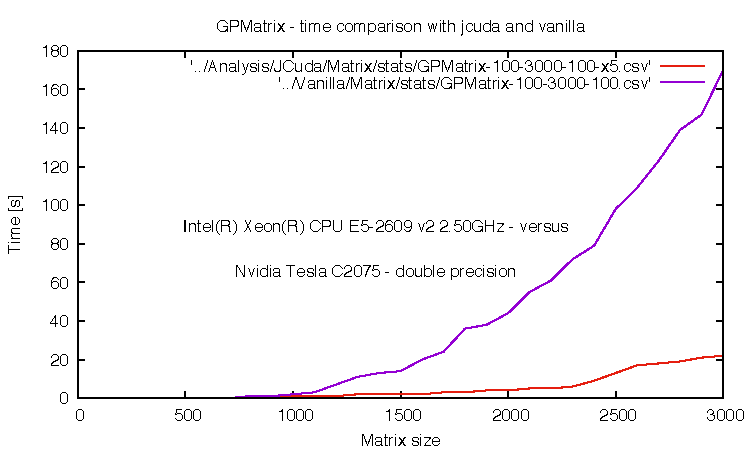
\includegraphics[width=1\textwidth]{time_jcuda_matrix_5x.pdf}
\caption{Times over matrix size using Java and JCuda}
\label{fig: plot jcuda matrix times}
\end{figure}

Figure \ref{fig table matrix jcuda} are some statistics on the speedup gained using JCuda. Those values will later be used to have metrics to compare between JCuda and Aparapi.

\begin{figure}[H]
\begin{center}
\begin{tabular}{ |l|l| } 
 \hline
 Speedup average & 5.6 \\ 
 Speedup median & 7 \\ 
 Speedup std. deviation & 4.3 \\ 
 \hline
\end{tabular}
\end{center}
\caption{Speedup statistics of matrix multiplication performed with JCuda}
\label{fig table matrix jcuda}
\end{figure}

\subsection{Levenshtein distance}

Figure \ref{fig plot leven jcuda} is the speedup gained using JCuda for the Levenshtein distance against vanilla code. The speedup gives its highest peak around a string size of 200'000 and decreases after. We observed the same behavior using Aparapi. Measures were based on an average of 5 executions and raw values are available in appendix \ref{raw values speedup jcuda Leven}. The uncertainty is discussed in appendix \ref{uncertain}. Full code can also be found in the appendix \ref{jcuda code}.

Unlike with the matrix multiplication, Aparapi gave a better peak with a speedup of nearly 80, while JCuda is around 55 at its highest peak.

\begin{figure}[H]
\centering
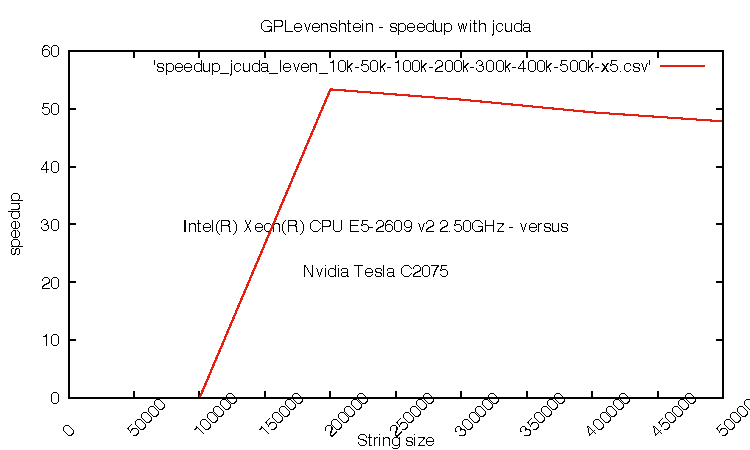
\includegraphics[width=1\textwidth]{speedup_jcuda_leven_5x.pdf}
\caption{Speedup gained using JCuda on Levenstein distance computation}
\label{fig plot leven jcuda}
\end{figure}

Figure \ref{fig: plot jcuda leven times} shows sequential times while executing the Levenshtein distance computation on different string sizes with JCuda and  vanilla Java, this on the same graph. Sequential times for JCuda are ridiculously small compared to the vanilla Java. Those measures are based on an average of 5 executions. Raw values of the execution times for the Levenstein distance computation using JCuda are available in appendix \ref{raw values jcuda leven}.

Statistics about the speedup are available in figure \ref{fig table leven jcuda}.

\begin{figure}[H]
\centering
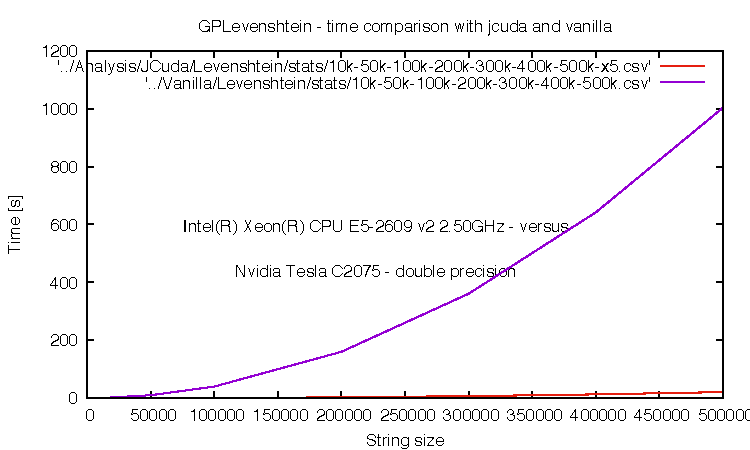
\includegraphics[width=1\textwidth]{time_jcuda_leven_5x.pdf}
\caption{Times over string size using Java and JCuda}
\label{fig: plot jcuda leven times}
\end{figure}

\begin{figure}[H]
\begin{center}
\begin{tabular}{ |l|l| } 
 \hline
 Speedup average & 28.5 \\ 
 Speedup median & 47.8 \\ 
 Speedup std. deviation & 24.8 \\ 
 \hline
\end{tabular}
\end{center}
\caption{Speedup statistics of Levenstein computation performed with JCuda}
\label{fig table leven jcuda}
\end{figure}

\subsection{External feedback}

We asked 2 developers to evaluate the difficulty of using JCuda to write GPU code. We gave them the Matrix multiplication and the Levenshtein distance source codes, asking them to give a mark from 1 (very difficult to understand) to 5 (very easy to understand). The surveys can be found in the appendix \ref{jcuda code}.

Results are given in the figure \ref{table jcuda code feedback}:

\begin{figure}[H]
\begin{center}
\begin{tabular}{ |l|l|l|l| } 
 \hline
  & \textbf{Matrix} & \textbf{Levenstein} \\
 \hline
 \textbf{Developper 1} & 4 & 3 \\ 
 \hline
 \textbf{Developper 2} & 4 & 3 \\ 
 \hline
\end{tabular}
\end{center}
\caption{Results of the JCuda surveys. From 1 (very difficult to understand) to 5 (very easy to understand)}
\label{table jcuda code feedback}
\end{figure}

\subsection{LOC}

The numbers of code lines needed to use JCuda for the matrix multiplication and Levenshtein distance computation are given in figure \ref{table jcuda loc}. Those numbers include only the methods used to compute the matrix multiplication and the Levenshtein distance, removing comments and blank lines.

\begin{figure}[H]
\begin{center}
\begin{tabular}{ |l|l|l|l| } 
 \hline
 & \textbf{vanilla} & \textbf{JCuda} & \textbf{delta} \\
 \hline
 \textbf{GPMatrix} & 13 & 47 & 30 \\ 
 \hline
 \textbf{GPLevenstein} & 18 & 51c & 25 \\ 
 \hline
\end{tabular}
\end{center}
\caption{LOC of GPMatrix and GPLevenstein using JCuda compared with vanilla}
\label{table jcuda loc}
\end{figure}

\subsection{Overall feedback}

JCuda is really well documented and easy to install. Due to its binding philosophy, using JCuda gives more the impression of writing CUDA code in Java than using Java to write GPU code. The fact that the kernel method is written in C is the main reason, but also the way we allocate and set the kernel's parameters. From Java, all we do is calling the kernel exactly as we would with CUDA, but with Java methods. This can be disturbing for someone who has no experience using CUDA, but on the other hand, if someone has already a CUDA experience, it won't be difficult at all to get started.

A major restriction of using JCuda is due to the kernel written in C. It does not allow developers to use Java code and breaks the process of a pure Java development workflow. This lets only the possibility to write a single c method. In our case, for example, we couldn't use or write a simple method \textbf{min()} that would make the code much easier to read in our kernel. But, in the other hand, an advantage of using the kernel in its pure form, written in C, is the fact that it makes possible to use already written CUDA kernel methods. Hence making the process of kernel reusability among other existing projects possible. This aspect should be worth considering in some context.

In conclusion, JCuda was easy to install, well documented and relatively fast to get started with. Using pure kernel methods in C could be interesting for someone familiar with CUDA, but does not have the advantage of using Java code. For Java code that needs to execute specific instructions to the GPU on a CUDA architecture, JCuda is a good solution as long as the kernel does not need any Java objects and/or methods.

\chapter{Results}
This chapter will finally compare Aparapi and JCuda based on the test battery we applied on them in the previous chapter.

As discussed in the introduction (see section \ref{goals}), our comparison is based on the execution speed and ease of use. We will discuss each comparison point for Aparapi and JCuda so as to evaluate which one is better for each criteria.

The next chapter will be an overall conclusion, bringing the final thoughts and perspectives.

\section{Execution speed}

For the execution speed, two benchmarks were used and executed against Aparapi and JCuda. The baseline used for the speedup were a native execution on a vanilla Java code using only the host's CPU.

Each benchmark is testing a different type of computation. The matrix multiplication is more focused on floating point operations while the Levenshtein distance is more focused on char operations.

For each benchmark, we will compare the speedup gained using Aparapi and JCuda.

\subsection{Matrix}

The following table is a side by side comparison of Aparapi and JCuda for the matrix multiplication, based on the speedup.

\renewcommand{\arraystretch}{2}
\begin{figure}[H]
\begin{tabular}[width=1\textwidth]{c|c}
	\textbf{Aparapi} & \textbf{JCuda} \\
	\hline \hline
	\multicolumn{2}{c}{Speedup plot} \\
	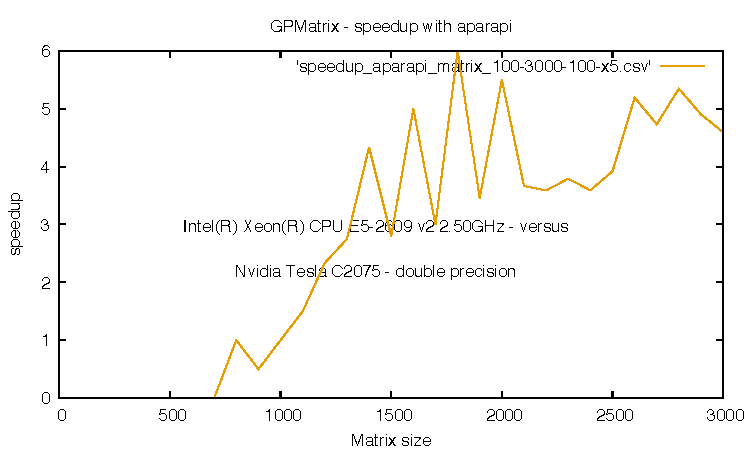
\includegraphics[width=.5\textwidth]{speedup_aparapi_matrix_5x.pdf} &
	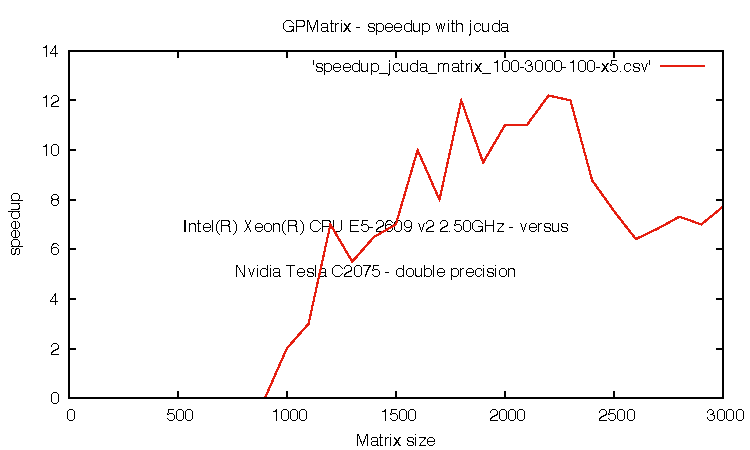
\includegraphics[width=.5\textwidth]{speedup_jcuda_matrix_5x.pdf} \\
	\hline
	\multicolumn{2}{c}{Speedup peak} \\
	\textcolor{BrickRed}{6} & \textcolor{OliveGreen}{\textbf{12.2}} \\
	\hline
	\multicolumn{2}{c}{Speedup average} \\
	\textcolor{BrickRed}{2.3} & \textcolor{OliveGreen}{\textbf{5.6}} \\
	\hline
	\multicolumn{2}{c}{Speedup median} \\
	\textcolor{BrickRed}{3.4} & \textcolor{OliveGreen}{\textbf{7}} \\
	\hline
	
\end{tabular}
\end{figure}

On this turn, JCuda shows a clear better performance on all the metrics, having globally an execution time 2 times faster than Aparapi. But it is worth noting that JCuda seems to suddenly decrease performance after a certain matrix size (around 2400), while Aparapi show a globally more stable speedup. But even with this consideration, JCuda always shows a better speedp.

\subsection{Levenshtein}

The following table is a side by side comparison of Aparapi and JCuda for the Levenstein distance computation, based on the speedup.

\begin{figure}[H]
\begin{tabular}[width=1\textwidth]{c|c}
	\textbf{Aparapi} & \textbf{JCuda} \\
	\hline \hline
	\multicolumn{2}{c}{Speedup plot} \\
	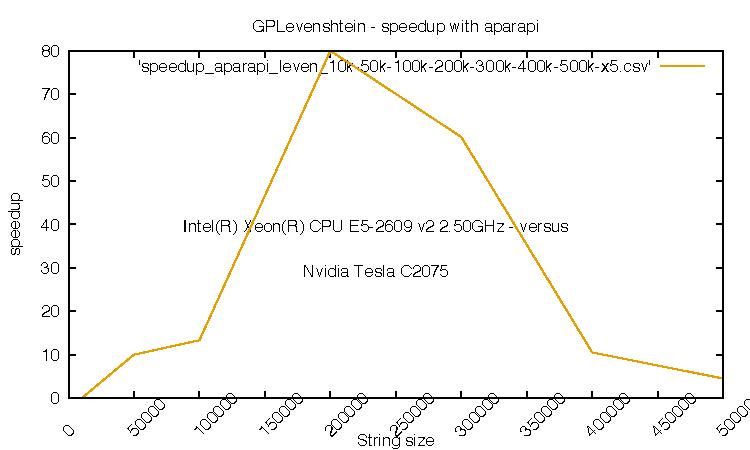
\includegraphics[width=.5\textwidth]{speedup_aparapi_leven_5x.pdf} &
	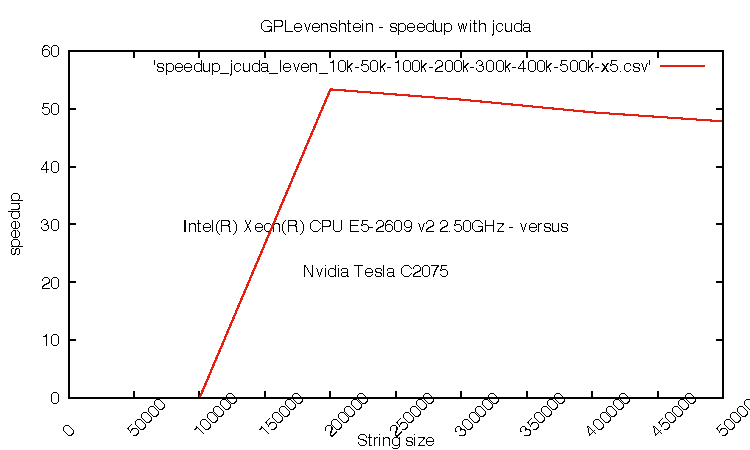
\includegraphics[width=.5\textwidth]{speedup_jcuda_leven_5x.pdf} \\
	\hline
	\multicolumn{2}{c}{Speedup peak} \\
	\textcolor{OliveGreen}{\textbf{80}} & \textcolor{BrickRed}{53.3} \\
	\hline
	\multicolumn{2}{c}{Speedup average} \\
	\textcolor{BrickRed}{25.2} & \textcolor{OliveGreen}{\textbf{28.5}} \\
	\hline
	\multicolumn{2}{c}{Speedup median} \\
	\textcolor{BrickRed}{10} & \textcolor{OliveGreen}{\textbf{47.8}} \\
	\hline
	
\end{tabular}
\end{figure}

Unlike with the matrix multiplication, this time we can't clearly define which solution is faster. Aparapi is globally less fast than JCuda but has the best peak with up to 80 times faster compared with JCuda - who has up to 53.3 times faster. The only answer we can give is "it depends". Around a string size of 200k, Aparapi is better than JCuda. But as soon as we have a bigger string size (around 300k), JCuda is a faster solution and shows a more stable speedup with an increasing string size. Based on the average speedup, JCuda is globally faster.

\section{Ease of use}

To evaluate the ease of use, we will be looking at the following aspects:
\begin{enumerate}
  \item The installation process
  \item The number of code lines
  \item The external feedbacks
  \item The problems encountered and restrictions
\end{enumerate}

\subsection{Installation process}

In both cases - with Aparapi and JCuda - the installation process were very similar and fast. Despite the fact that we didn't have any difficulties getting started and installing both of the solutions, we give the medal to JCuda for this turn.

JCuda was easier to instal due to a better documentation, providing examples and command lines to compile and execute a JCuda based program. This support wasn't as good with Aparapi, where we didn't really find any good getting started explanation.

\subsection{Line of codes}

The following table is a side by side comparison of Aparapi and JCuda concerning the line of codes needed to run the matrix multiplication and Levenshtein distance computation. In parenthesis are the differences with the number of code lines for the vanilla Java implementation.

\newcolumntype{Y}{>{\centering\arraybackslash}X}
\begin{figure}[H]
\begin{tabularx}{\textwidth}{@{}Y|Y|Y@{}}
	\textbf{Aparapi} & \textbf{JCuda} & \textbf{(Vanilla)} \\
	\hline \hline
	\multicolumn{3}{c}{Matrix multiplication} \\
	\textcolor{OliveGreen}{\textbf{21} (+8)} & \textcolor{BrickRed}{47 (+34)} & 13 \\
	\hline
	\multicolumn{3}{c}{Levenstein distance computation} \\
	\textcolor{OliveGreen}{\textbf{24} (+6)} & \textcolor{BrickRed}{51 (+38)} & 18 \\
	\hline
	
\end{tabularx}
\end{figure}

Aparapi wins by far this turn with more than 2 times less lines of code needed to perform the same task than with JCuda.

Aparapi was much easier to implement in terms of code lines needed. This difference with JCuda is mainly due to the need for JCuda to set each kernel attribute so it is available to the kernel method - which is written in C. This process requires many steps. For a quick use, Aparapi is more suitable than JCuda.

\subsection{External feedback}

The following table summarizes the external feedback on how developers evaluated the difficulty to understand the code - especially the part performing computation on the GPU. They had to give a mark from 1 (very difficult) to 5 (very easy). In the following table are the averages' marks.

\newcolumntype{Y}{>{\centering\arraybackslash}X}
\begin{figure}[H]
\begin{tabularx}{\textwidth}{@{}Y|Y|Y@{}}
	\textbf{Aparapi} & \textbf{JCuda} \\
	\hline \hline
	\multicolumn{2}{c}{Matrix multiplication - external developers feedback average marks} \\
	\textcolor{OliveGreen}{\textbf{5}} & \textcolor{BrickRed}{3.5} \\
	\hline
	\multicolumn{2}{c}{Levenstein distance - external developers average feedback marks} \\
	\textcolor{OliveGreen}{\textbf{5}} & \textcolor{BrickRed}{3.5} \\
	\hline
	
\end{tabularx}
\end{figure}

Aparapi seems to be more easier to understand than JCuda. It is probably due to the fact that JCuda requires more lines of code and a kernel written in C. The external feedback were performed with 2 developers having already an experience in GPU programming.

\subsection{Problems encountered - restrictions}

\begin{figure}[H]
\begin{tabularx}{\textwidth}{@{}Y|Y@{}}
	\textbf{Aparapi} & \textbf{JCuda} \\
	\hline \hline
	 
	 \begin{itemize}
	   \item
	   No official getting started guide found. We had to use examples so as to start using Aparapi.
       \item 
       Impossible to use any Java objects inside the kernel method. We had to write our own min() methods and convert strings to char arrays. 
       \item
       Impossible to get the size of an array inside the kernel. It is a known issue \cite{aparapibug}.
     \end{itemize} 
     
     &

	 \begin{itemize}
       \item Like Aparapi, impossible to use Java objects but even any Java code inside the kernel method.
       \item The kernel method is written in C, not in Java. This restricts the use of Java but makes the reusability and sharing of existing CUDA kernel methods possible.
       \item Impossible to write a simple min() method for the kernel, making the code hard to read.
     \end{itemize} \\

	\hline
	
\end{tabularx}
\end{figure}
\renewcommand{\arraystretch}{1}

In terms of restrictions, we can't clearly give a single medal to Aparapi or JCuda. The answer is "it depends". Either Aparapi or JCuda can't use Java objects in the kernel methods. Aparapi has the advantage of being fully usable under a Java workflow, while JCuda needs a kernel written in C. Aparapi gives the ability to have custom methods available from the kernel, giving more flexibility. On the other hand, JCuda has it's kernel written in C, giving the ability to use already written CUDA kernel methods. This also makes the use of JCuda from someone already knowing CUDA easy, since the kernel code remains the same, and the process, for JCuda, of calling the kernel method is also very similar as one we would do with vanilla CUDA programming.

For someone already knowing CUDA, JCuda gives a better way to use the GPU from a Java code. But this only under a CUDA compatible environment.

For someone looking for a full Java solution to write GPU code, having an OpenCL environement and giving the ability to write flexible methods available from the kernel, Aparapi is a better solution.

\chapter{Conclusion}
This chapter is the final words that will conclude our analysis of Aparapi and JCuda.

\section{Aparapi or JCuda?}

For someone absolutely looking for the fastest solution, JCuda is more suitable than Aparapi. In our analysis, based on a matrix multiplication and a Levenshtein distance, JCuda is globally faster than Aparapi, with sometimes results more than 2 times faster than Aparapi. However, we observed one case on a particular string size for the Levenshtein distance computation where Aparapi was faster. So, even speaking of speed, Aparapi could be faster on particular cases. Globally, JCuda is faster but we couldn't test every cases on every computation types.

Speaking about ease of use, Aparapi wins the palm and is more suitable than JCuda. It requires less line of codes, has the advantage of being entirely usable in Java and doesn't need an CUDA environment, which is not always possible for someone not having an NVDIA GPU.

JCuda requires a kernel written in C, which could be either an advantage or a disadvantage. Someone already familiar with JCuda won't have any difficulties since the kernel whould be the same, but for someone not familiar with CUDA programming it will be more difficult to get started compared to Aparapi.

If keeping an absolute Java environment is a priority, Aparapi comes as the only possible solution. With Aparapi, everything is written in Java, providing a smooth development workflow and a clear code. It also gives the abilities of writing custom Java methods helper available from the kernel - which is not possible with JCuda.

\section{The answer}

Answering the question "should I use Aparapi od JCuda?" requires to know what are the needs and the development environment available. It maily requires to answer three questions :

\begin{enumerate}
  \item Do we have a CUDA or OpenCL environment?
  \item Do I want to keep the code simple and stay exclusively with Java?
  \item Am I focused on speed?
\end{enumerate}

The process to guide the choice of Aparapi or JCuda based on the previous questions is given by the flowchart in the figure \ref{fig: flow final choice}.

\begin{figure}[h]
\centering
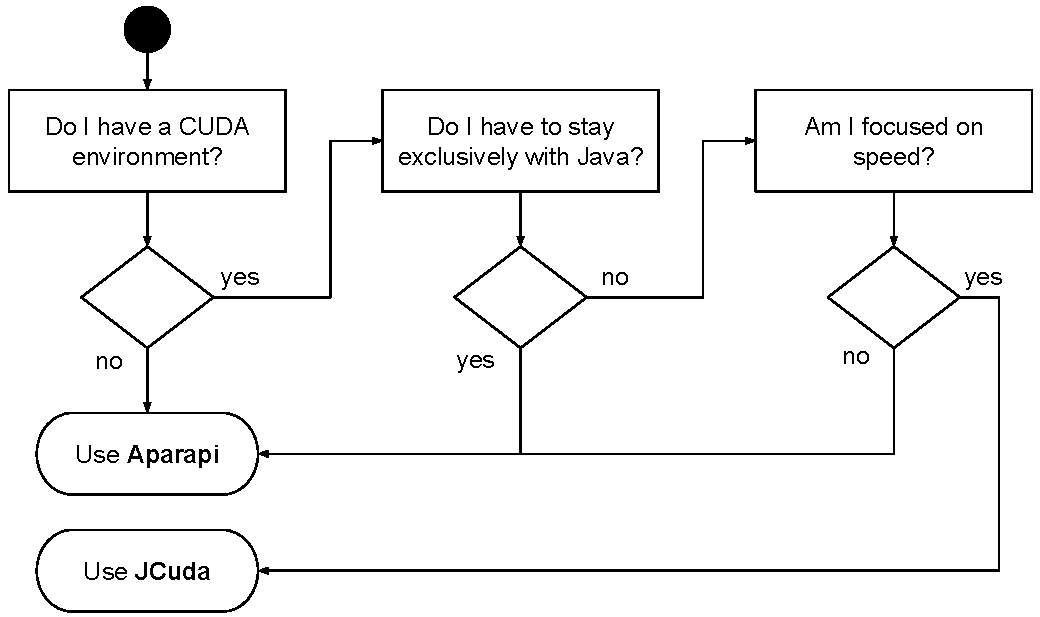
\includegraphics[width=1\textwidth]{final_flow}
\caption{Flowchart guiding the decision of using either Aparapi or JCuda}
\label{fig: flow final choice}
\end{figure}

However, this process may not be true on every cases, especially speaking of speed where Aparapi could be faster on some cases - and we obviously couldn't test every cases for every computation types. We are only saying that JCuda is globally faster, but there could be cases where it is not. The last question on the flow "Am I focused on speed?" could lead to JCuda even if the answer is "no" for someone who prefers using a CUDA based solution anyway. At this point of the flow, it is more a question of flavor. We tried, on the flow, to fit the most global use case and answer the question for, what we think, corresponds to the majority.

\section{Perspectives}

There are some points that could be expanded and leave some future perspectives. We are thinking of :

\begin{itemize}
  \item Testing more solutions
  \item Developping more benchmarks
  \item Increasing the measures' precisions
\end{itemize}

Aparapi and JCuda are of course not the only solutions that make GPU programming available from Java. In our pre-analysis (see table \ref{pre analysis}), we had 11 candidates and we only evaluated 2 of them. We chose the first 2 of them that seemed the most promising to us, but evaluating more of them according to our test battery could lead us to better solutions.

Our test battery only uses 2 benchmarks. Having more benchmarks would give us more specific measures about what solution is the best for what kind of computation and parameter. As we saw, JCuda is globally faster than Aparapi. But in special cases, Aparapi is faster. With more benchmarks we would perhaps discover more special cases where Aparapi is  faster, and then giving a more precise way to make a decision between Aparapi and JCuda.

Our benchmark only measures the rounded seconds spent. Hense, the sequential time and the speedup suffer from an uncertainty that could be important in some cases. The uncertainty in our measures is discussed in appendix \ref{uncertain}. The uncertainty could be much reduced by measuring the sequential time in milliseconds instead of rounded seconds.

\printbibliography

\chapter*{Declaration of Authorship}
I hereby certify that the paper I am submitting is entirely my own original work except
where otherwise indicated. I am aware of the regulations concerning
plagiarism, including those regulations concerning disciplinary actions that may result
from plagiarism. Any use of the works of any other author, in any form, is properly
acknowledged at their point of use.

\bigskip
\bigskip

Place \hfil Date \hfil Signature

\appendix
\chapter{Source code structure}
Official repository address: https://github.com/nkcr/JavaGPU \\

This is the list of the four root folders and their contents : \\

\renewcommand{\arraystretch}{2}
\begin{tabular}{ l|l } 
 \hline
 \textbf{Analysis} & Code and measures using different Java GPU technologies \\
 \hline
 \textbf{Common} & Common stuff needed across the project like libraries \\ 
 \hline
 \textbf{Results} & Contains comparison measures like speedup \\ 
 \hline
 \textbf{Vanilla} & Code written in pure Java so as to have base metrics \\ 
 \hline
\end{tabular}
\renewcommand{\arraystretch}{1}

\chapter{Versions used}
\renewcommand{\arraystretch}{2}
\begin{tabular}{ l|l } 
 \hline
 \textbf{Java} & 1.7.0\_95 \\
 \hline
 \textbf{CUDA} & 7.5.18 \\ 
 \hline
 \textbf{OpenCL} & Platform: NVIDIA CUDA, version 1.1 \\ 
 \hline
 \textbf{JCuda} & 0.7.5 for CUDA 7.5.18 \\ 
 \hline
 \textbf{Aparapi} & 1.0.0 linux x86\_64 \\ 
 \hline
 \textbf{Ubuntu} & Ubuntu 14.04.4 LTS \\ 
 \hline
 \textbf{Bash} & RELEASE: 2.1 \\ 
 \hline
 \textbf{GNUplot} & Version 4.6 patchlevel 4 \\ 
 \hline
\end{tabular}
\renewcommand{\arraystretch}{1}

\chapter{List of initial candidates} \label{candidates}
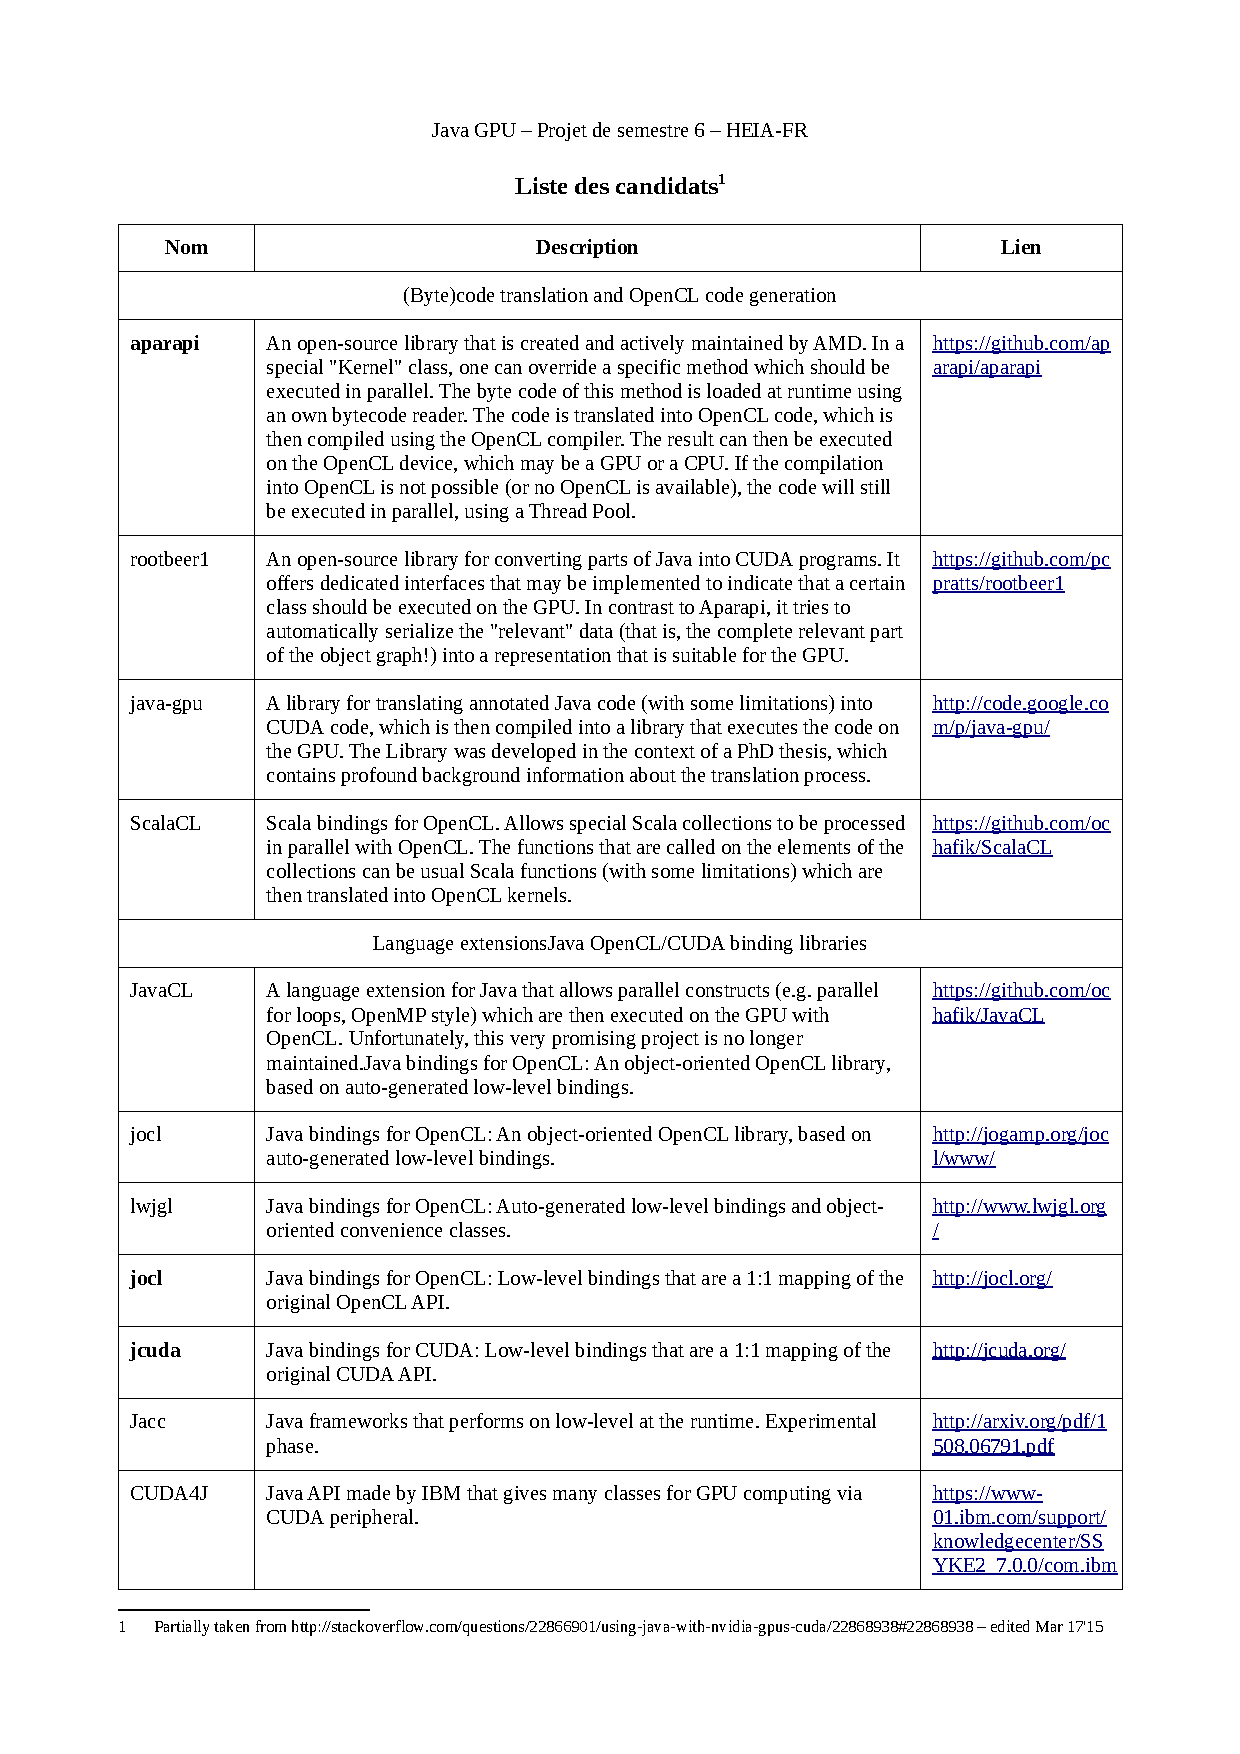
\includepdf[pages=-]{Listedescandidats.pdf}

\chapter{Installation of CUDA in Ubuntu 14.04}
\begin{lstlisting}
$ wget http://developer.download.nvidia.com/compute/cuda/repos/ubuntu1404/x86_64/cuda-repo-ubuntu1404_7.5-18_amd64.deb
$ sudo apt-get update
$ sudo apt-get install cuda
$ export CUDA_HOME=/usr/local/cuda-7.5 
$ export LD_LIBRARY_PATH=${CUDA_HOME}/lib64 
 
$ PATH=${CUDA_HOME}/bin:${PATH} 
$ export PATH
	
$ wget http://us.download.nvidia.com/XFree86/Linux-x86_64/352.79/NVIDIA-Linux-x86_64-352.79.run
$ chmod +x NVIDIA-Linux-x86_64-352.79.run
$ sudo ./NVIDIA-Linux-x86_64-352.79.run
	
$ cuda-install-samples-7.5.sh ~/cuda
$ cd ~cuda/NVIDIA_CUDA-7.5_Samples 
$ cd 1_Utilities/deviceQuery 
$ make
	
\end{lstlisting}

For the driver to be installed, Xserver must be disabled :

\begin{lstlisting}
# /etc/default/grub
$ GRUB_CMDLINE_LINUX_DEFAULT="text"
\end{lstlisting}

\chapter{Uncertainty discussed} \label{uncertain}
This appendix is a post-reflection on how the uncertainty impacts our results.

All our measures were made in rounded seconds, this means that all our data suffer from an uncertainty that could impact the results and the conclusions made. We will compute the uncertainty and re-plot the speedups that were used in this report, but this time showing the uncertainty.

First, let's find the formula giving the uncertainty. For a single measured value, say 10 seconds, we know that is has been rounded. It could be in reality 10.1 seconds, 10.5 seconds or, the maximum, 10.999999 seconds. Thus, the measure could be in reality from 10 seconds to 10.9999 seconds. Therefor, we have an uncertainty of maximum +1 seconds.

Based on this principle, we computed the uncertainty of the speedup ($S$) based on two measures ($x_1$, $x_2$) :

\[ S = \frac{x_1}{x_2} \]

\[ S_{max} = \frac{x_1+1}{x_2} \]

\[ S_{min} = \frac{x_1}{x_2+1} \]

\[ S_{uncertainty} = S_{max} - S_{min} = \frac{x_1+1}{x_2} - \frac{x_1}{x_2+1} = \frac{x_1+x_2+1}{x_2^2+x_2} \]

Given the previous formula, we re-plotted the speedup with the uncertainty. Figures \ref{fig: plot both matrix uncertain} and \ref{fig: plot both leven uncertain} show speedups of Aparapi and JCuda on the matrix multiplication and Levenshtein distance respectively with the uncertainty. We can see that the uncertainty should explain why the plots are not regular and smooth. Fortunately for us, the uncertainty is not great enough to impact the conclusions made. JCuda is still faster on most cases than Aparapi, even taking into account the incertainty.

\begin{figure}[H]
\centering
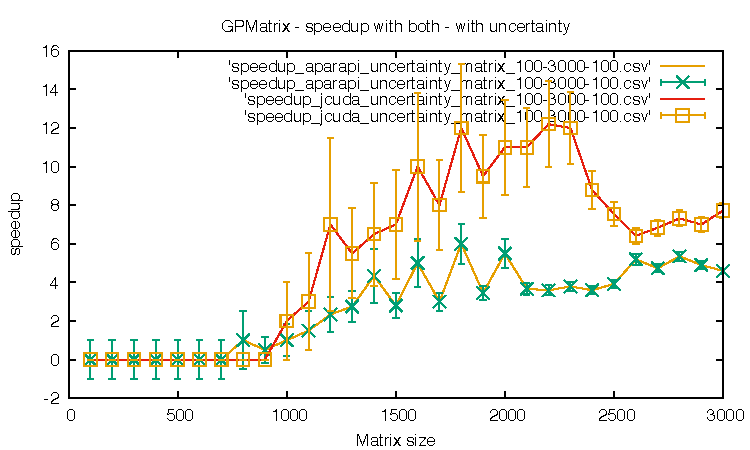
\includegraphics[width=1\textwidth]{speedup_both_uncertainty_matrix-5x.pdf}
\caption{Speedup of both Aparapi and JCuda on the matrix multiplication, showing uncertainty}
\label{fig: plot both matrix uncertain}
\end{figure}

\begin{figure}[H]
\centering
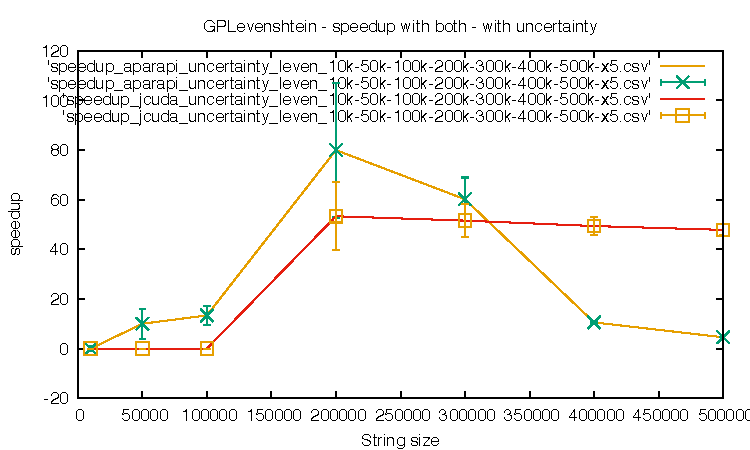
\includegraphics[width=1\textwidth]{speedup_both_uncertainty_leven-5x.pdf}
\caption{Speedup of both Aparapi and JCuda on the Levenstein distance computation, showing uncertainty}
\label{fig: plot both leven uncertain}
\end{figure}

\chapter{Raw values}
This appendix contains the raw values used for the plots in this document.

\section{Quick mesasure - matrix} \label{raw values quick matrix}

On a single execution. Double precision on an Intel(R) Xeon(R) CPU E5-2609 v2 2.50GHz.

\begin{tabular}{|c|c|}
  \hline
  \bfseries Matrix size & \bfseries Execution time [s]
  \csvreader{csv/quick-GPMatrix-100-3000-100.csv}{}
    {\\\hline\csvcoli&\csvcolii}
  \\\hline
\end{tabular}

\section{Quick measure - Leven} \label{raw values quick leven}

On a single execution. On an Intel(R) Xeon(R) CPU E5-2609 v2 2.50GHz.

\begin{tabular}{|c|c|}
  \hline
  \bfseries String size & \bfseries Execution time [s]
  \csvreader{csv/quick-10k-50k-100k-200k-300k-400k-500k.csv}{}
    {\\\hline\csvcoli&\csvcolii}
  \\\hline
\end{tabular}

\section{Aparapi - matrix} \label{raw values aparapi matrix}

Average of 5 executions. Double precision - Nvidia Tesla C2075.

\begin{tabular}{|c|c|}
  \hline
  \bfseries Matrix size & \bfseries Execution time [s]
  \csvreader{csv/aparapi-GPMatrix-100-3000-100-x5.csv}{}
    {\\\hline\csvcoli&\csvcolii}
  \\\hline
\end{tabular}

\section{Aparapi - Leven} \label{raw values aparapi leven}

Average of 5 executions. Nvidia Tesla C2075.

\begin{tabular}{|c|c|}
  \hline
  \bfseries String size & \bfseries Execution time [s]
  \csvreader{csv/aparapi-10k-50k-100k-200k-300k-400k-500k-x5.csv}{}
    {\\\hline\csvcoli&\csvcolii}
  \\\hline
\end{tabular}

\section{JCuda - matrix} \label{raw values jcuda matrix}

Average of 5 executions. Double precision - Nvidia Tesla C2075.

\begin{tabular}{|c|c|}
  \hline
  \bfseries Matrix size & \bfseries Execution time [s]
  \csvreader{csv/jcuda-GPMatrix-100-3000-100-x5.csv}{}
    {\\\hline\csvcoli&\csvcolii}
  \\\hline
\end{tabular}

\section{JCuda - Leven} \label{raw values jcuda leven}

Average of 5 executions. Nvidia Tesla C2075.

\begin{tabular}{|c|c|}
  \hline
  \bfseries String size & \bfseries Execution time [s]
  \csvreader{csv/jcuda-10k-50k-100k-200k-300k-400k-500k-x5.csv}{}
    {\\\hline\csvcoli&\csvcolii}
  \\\hline
\end{tabular}

\section{Speedup Aparapi matrix} \label{raw values speedup aparapi matrix}

Average of 5 executions. Nvidia Tesla C2075 versus Intel(R) Xeon(R) CPU E5-2609 v2 2.50GHz.

\begin{tabular}{|c|c|}
  \hline
  \bfseries Matrix size & \bfseries Speedup
  \csvreader{csv/speedup_aparapi_matrix_100-3000-100-x5.csv}{}
    {\\\hline\csvcoli&\csvcolii}
  \\\hline
\end{tabular}

\section{Speedup Aparapi Leven} \label{raw values speedup aparapi Leven}

Average of 5 executions. Nvidia Tesla C2075 versus Intel(R) Xeon(R) CPU E5-2609 v2 2.50GHz.

\begin{tabular}{|c|c|}
  \hline
  \bfseries String size & \bfseries Speedup
  \csvreader{csv/speedup_aparapi_leven_10k-50k-100k-200k-300k-400k-500k-x5.csv}{}
    {\\\hline\csvcoli&\csvcolii}
  \\\hline
\end{tabular}

\section{Speedup JCuda matrix} \label{raw values speedup jcuda matrix}

Average of 5 executions. Nvidia Tesla C2075 versus Intel(R) Xeon(R) CPU E5-2609 v2 2.50GHz.

\begin{tabular}{|c|c|}
  \hline
  \bfseries Matrix size & \bfseries Speedup
  \csvreader{csv/speedup_jcuda_matrix_100-3000-100-x5.csv}{}
    {\\\hline\csvcoli&\csvcolii}
  \\\hline
\end{tabular}

\section{Speedup JCuda Leven} \label{raw values speedup jcuda Leven}

Average of 5 executions. Nvidia Tesla C2075 versus Intel(R) Xeon(R) CPU E5-2609 v2 2.50GHz.

\begin{tabular}{|c|c|}
  \hline
  \bfseries String size & \bfseries Speedup
  \csvreader{csv/speedup_jcuda_leven_10k-50k-100k-200k-300k-400k-500k-x5.csv}{}
    {\\\hline\csvcoli&\csvcolii}
  \\\hline
\end{tabular}

\chapter{Vanilla matrix measure comparison} \label{vanilla matrix both}
The following plot (figure \ref{fig plot matrix both}) is a comparison of the base values taken as a reference for the  test battery concerning the matrix multiplication on a vanilla Java code.

On the graph is plotted the base values used to compute the speedup and a measure based on the average of 5 executions. This plot demonstrates that no edge cases happened while taking the base values. The two plots show a similar behavior and even sometimes the same values.

It is worth noting that the second measure took place 2 weeks after the first one.

\begin{figure}[h!]
\centering
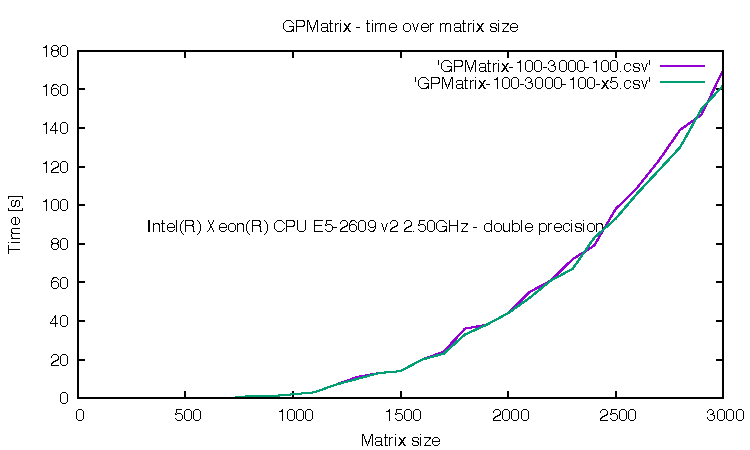
\includegraphics[width=1\textwidth]{vanilla_matrix_both.pdf}
\caption{Comparison of the base value with a measure performing an average on 5 executions.}
\label{fig plot matrix both}
\end{figure}

\chapter{External feedback survey for Aparapi} \label{aparapi code}

This appendix contains the feedback sheets used to evaluate Aparapi on the matrix multiplication and the Levenshtein distance computation respectively.
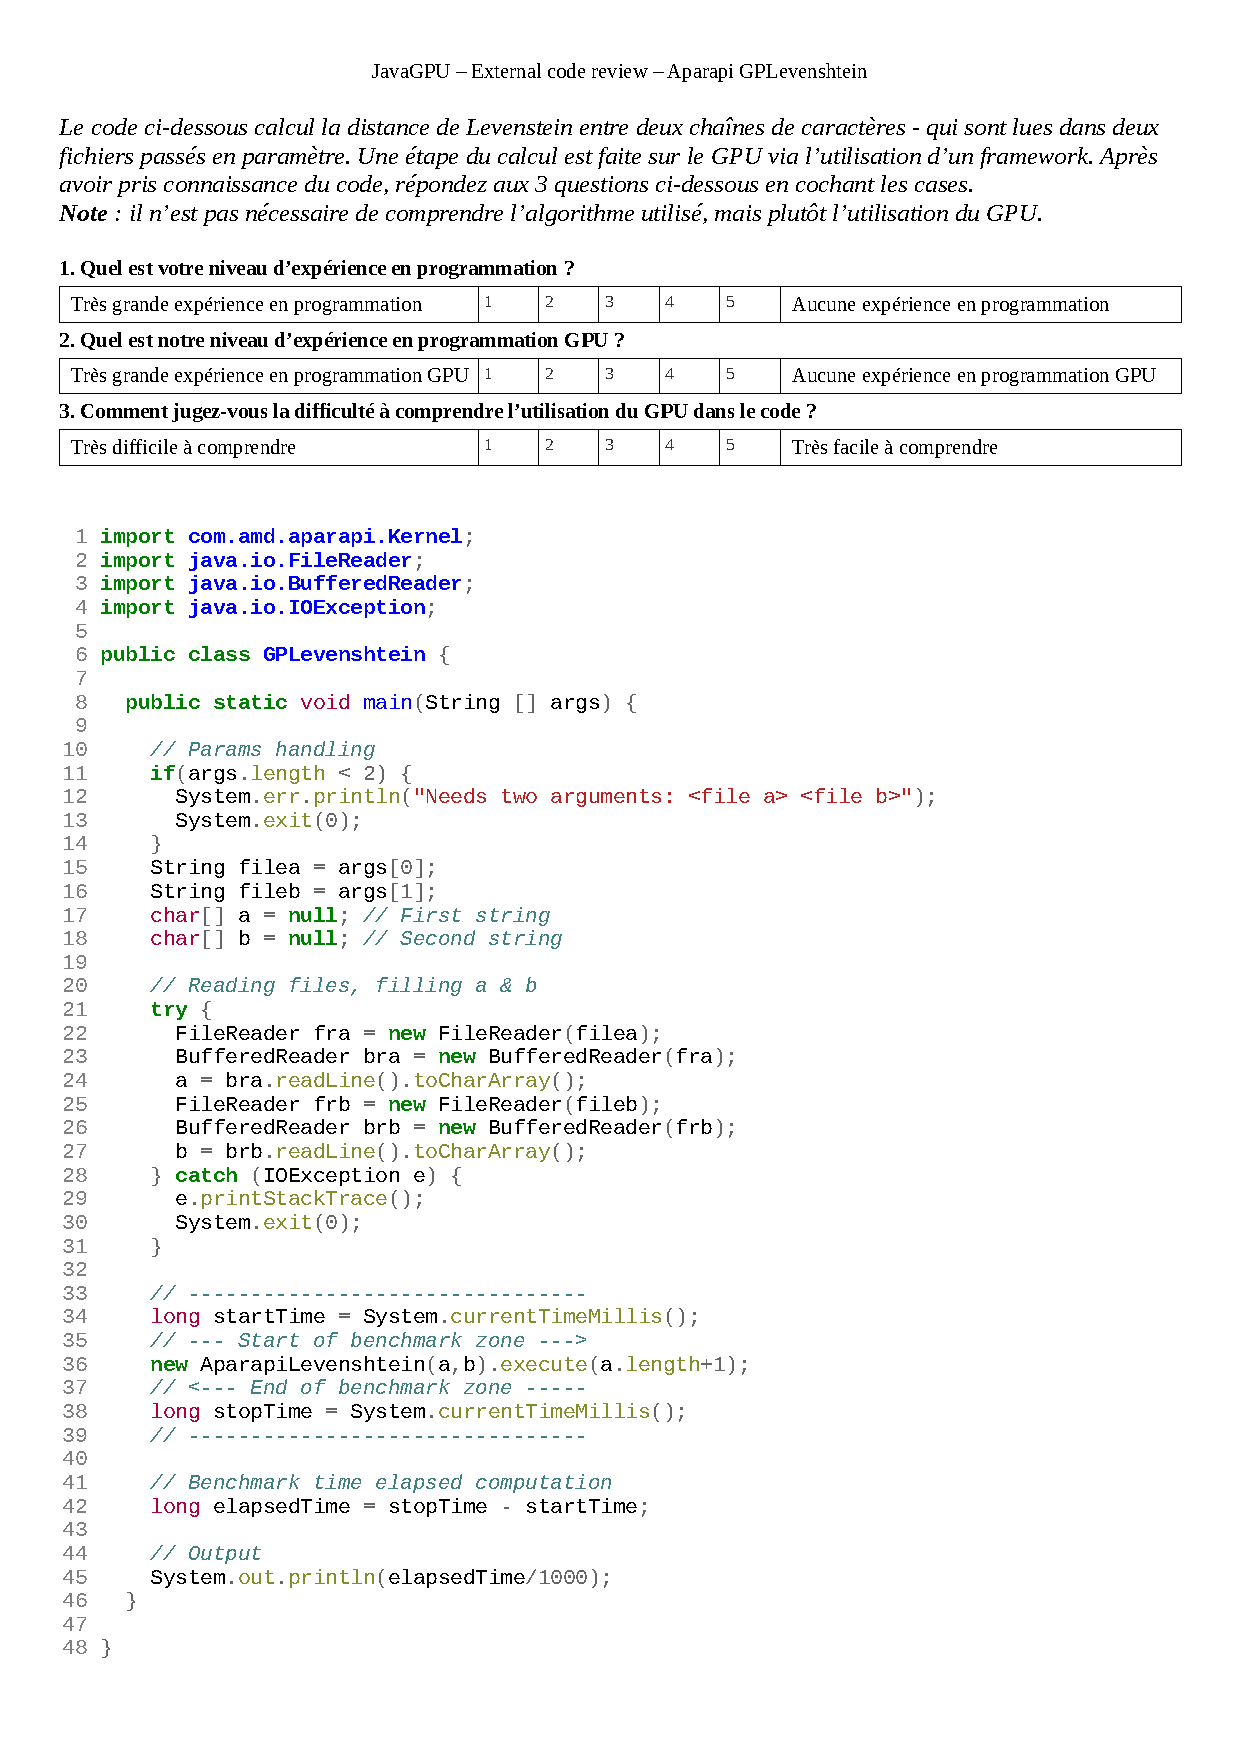
\includepdf[pages=-]{appendix/Aparapi_leven.pdf}
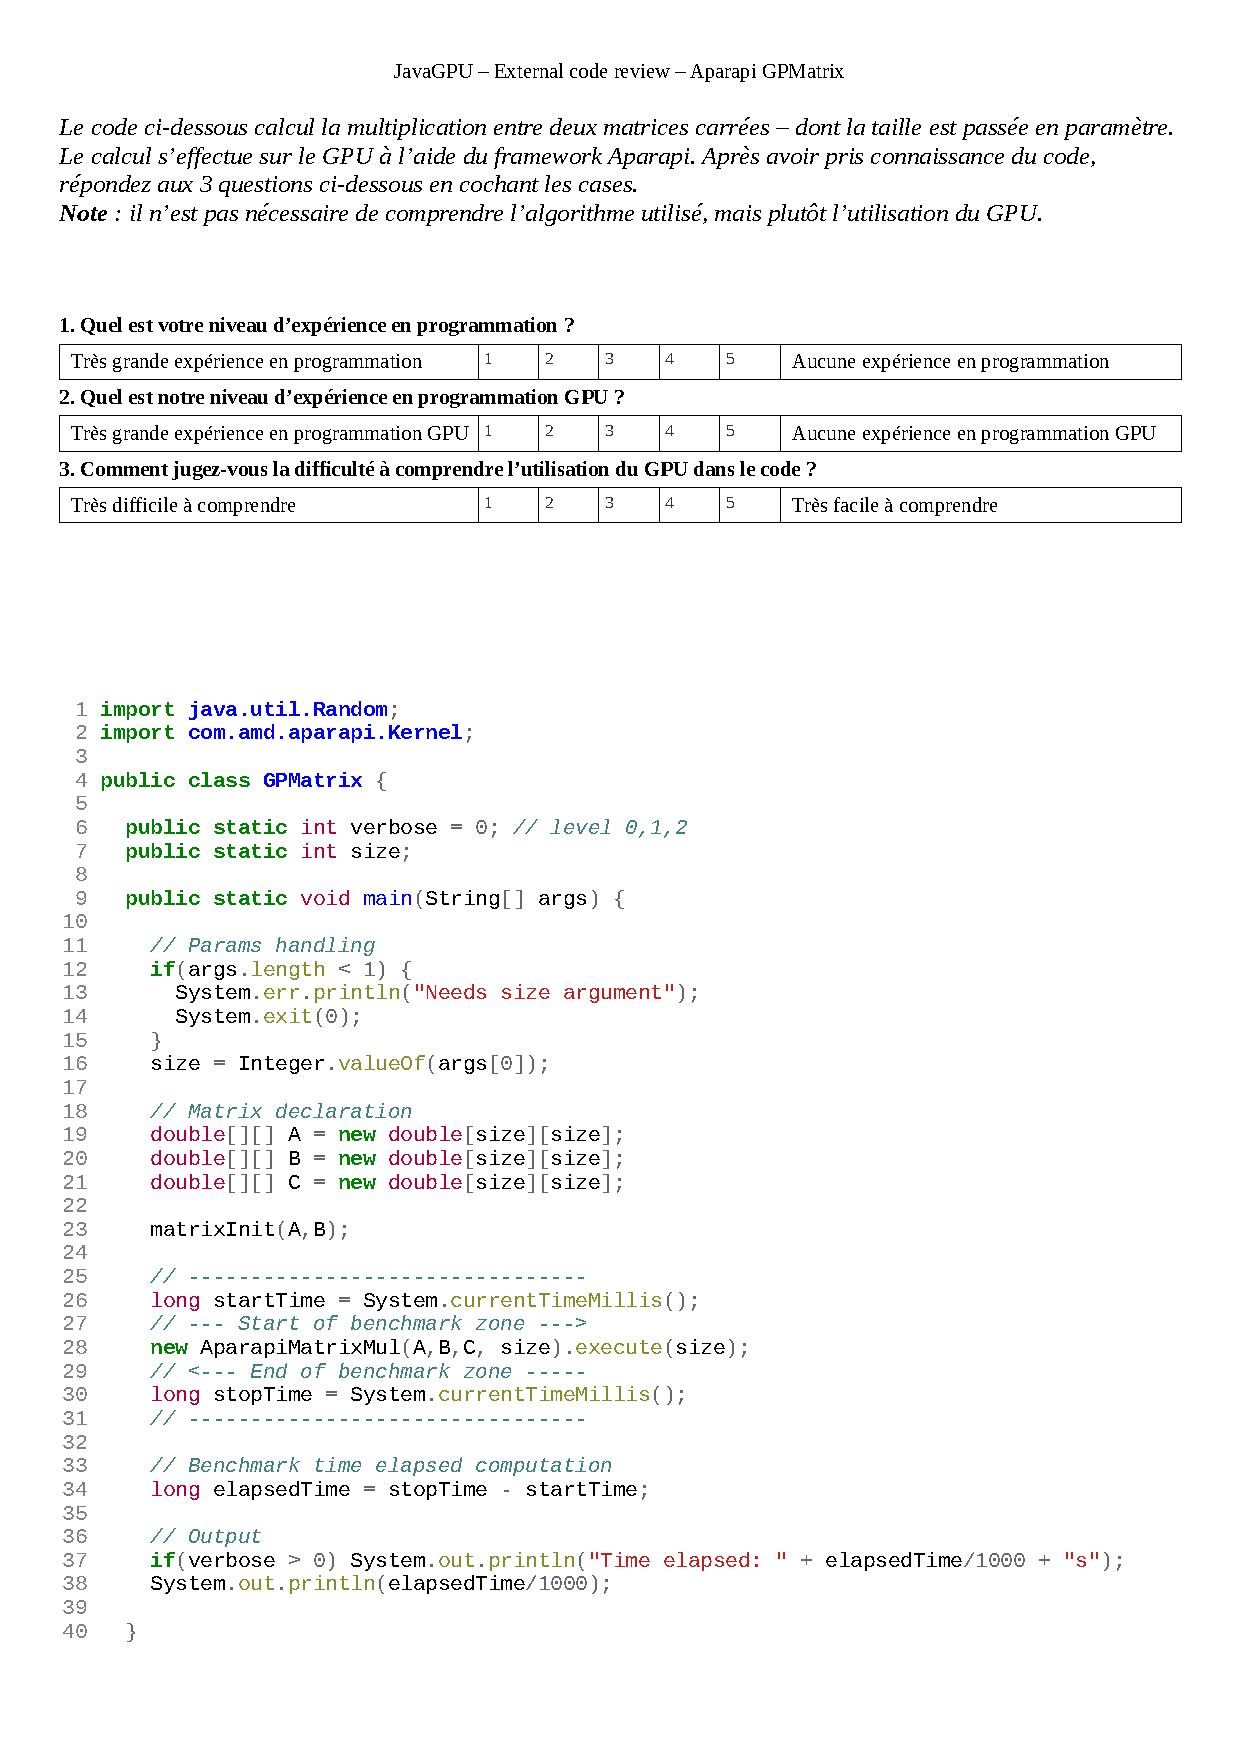
\includepdf[pages=-]{appendix/Aparapi_matrix.pdf}

\chapter{External feedback survey for JCuda} \label{jcuda code}

This appendix contains the feedback sheets used to evaluate JCuda on the matrix multiplication and the Levenshtein distance computation respectively.

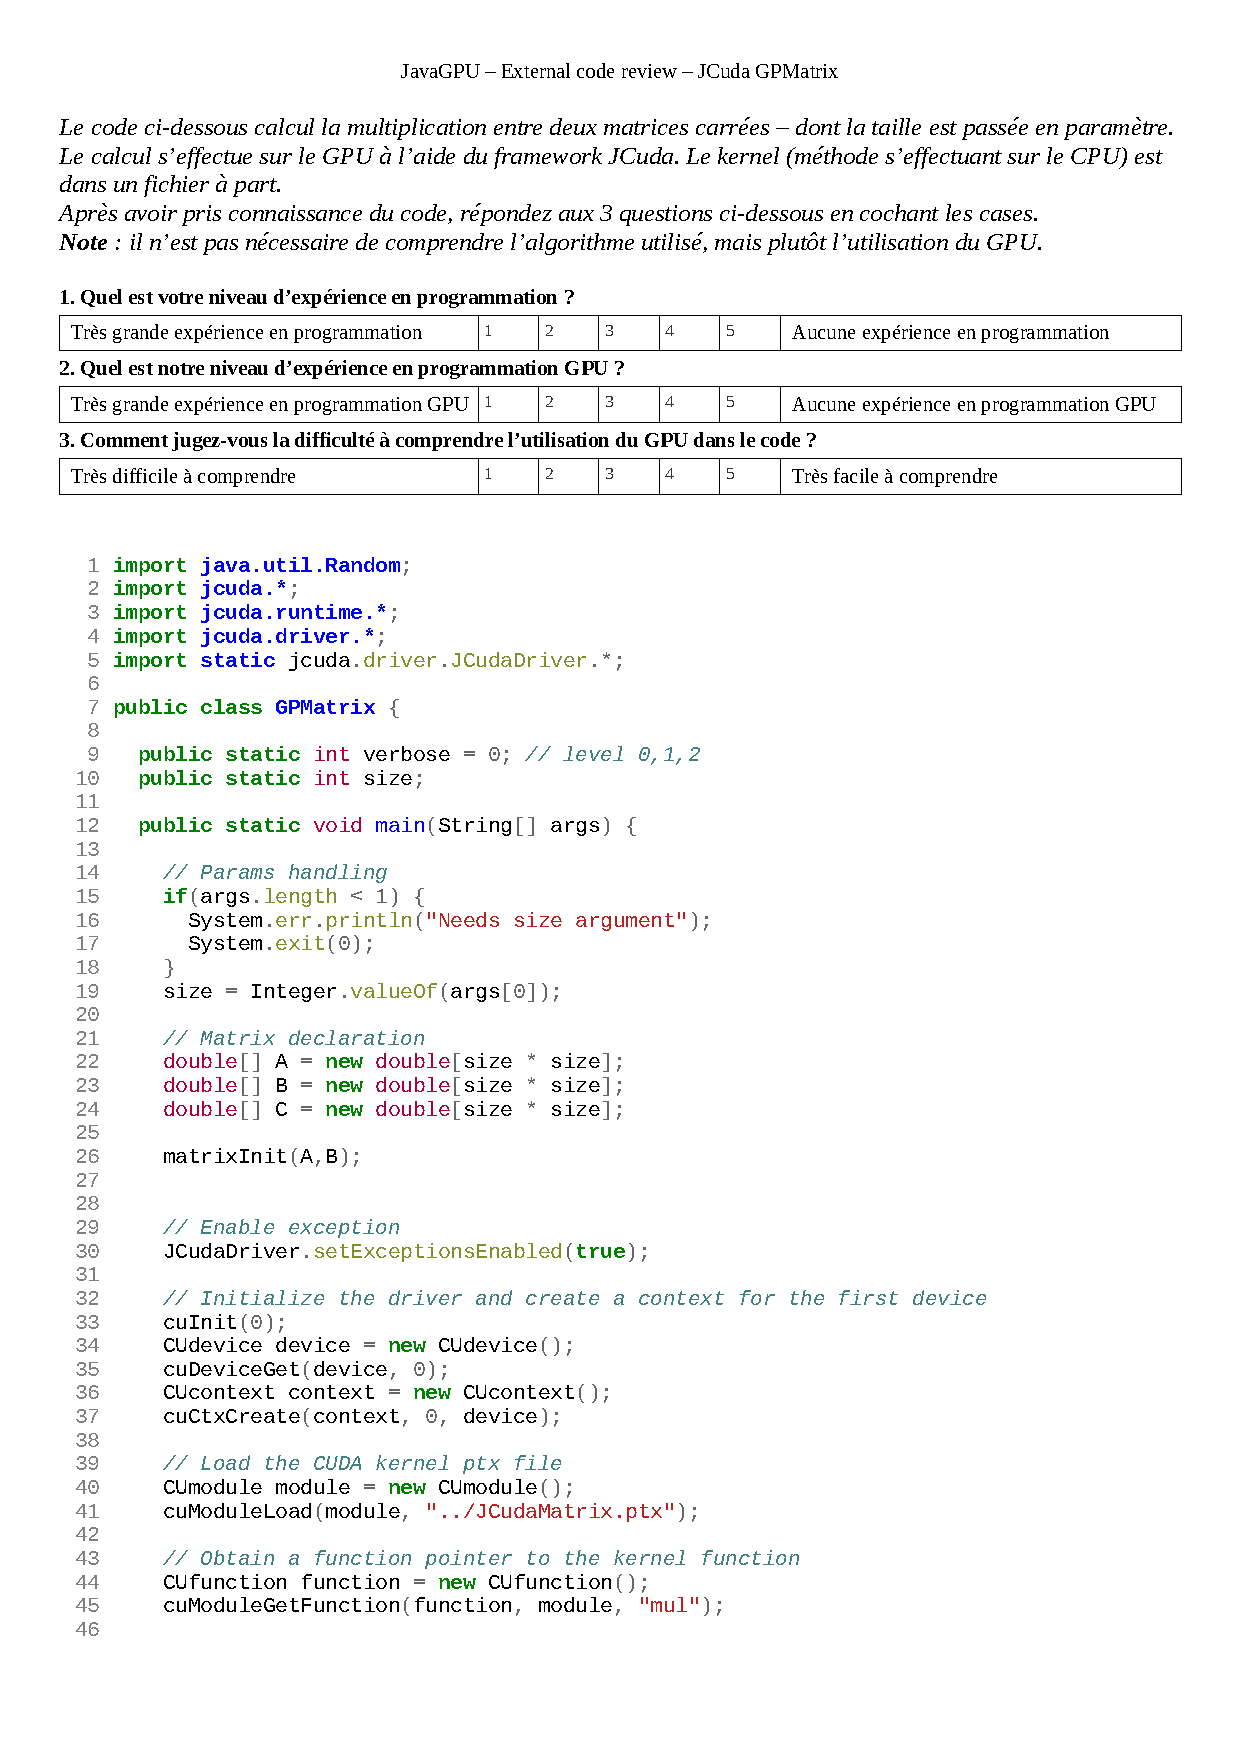
\includepdf[pages=-]{appendix/JCuda_matrix.pdf}
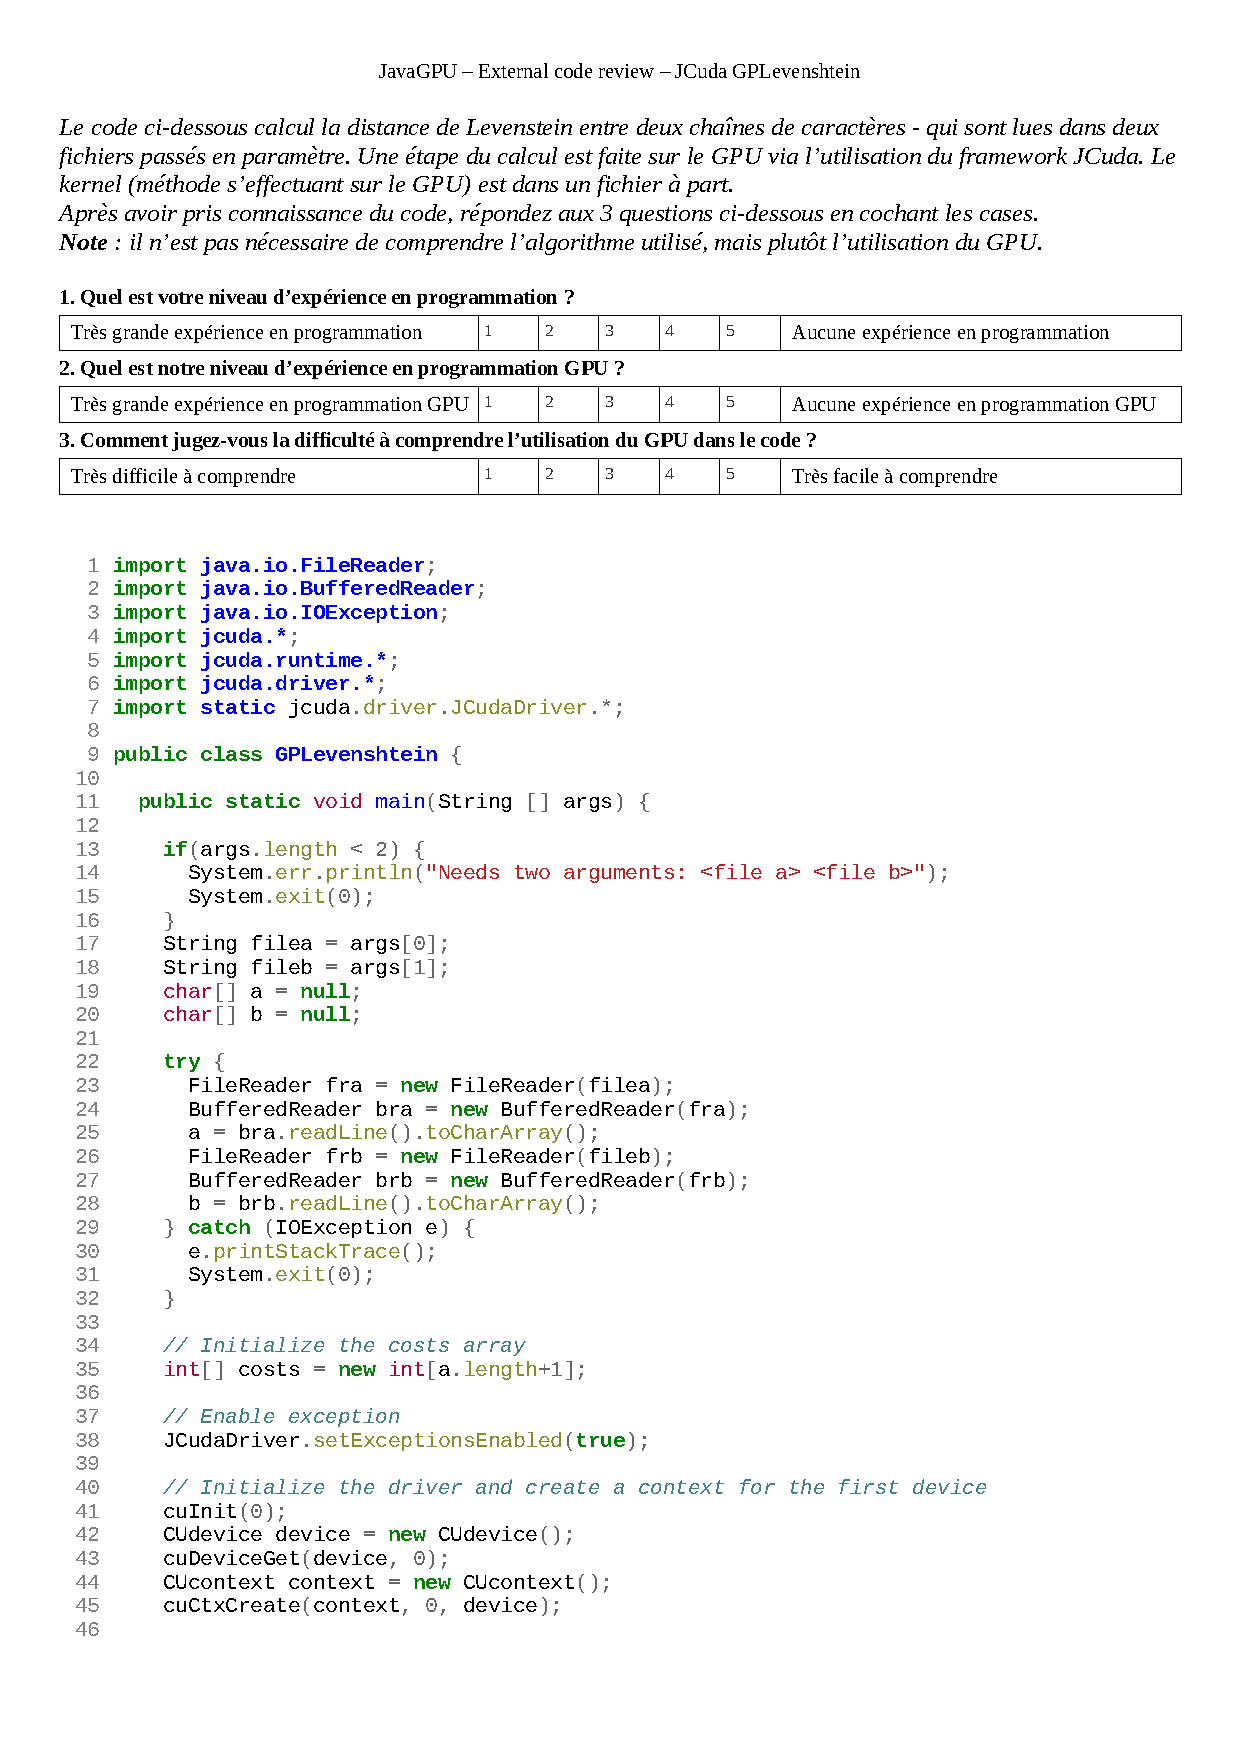
\includepdf[pages=-]{appendix/JCuda_leven.pdf}

\end{document}

% https://www.sharelatex.com/blog/2013/08/02/thesis-series-pt1.htmlx